\documentclass[journal]{IEEEtran}
\usepackage{amsmath,amsthm} % before newtxmath, which also provides the AMS symbols
\usepackage{iftex}
\ifXeTeX % e.g. Tectonic: Times text via TeX Gyre Termes
  \usepackage{newtxmath}
  \usepackage[no-math]{fontspec}
  \setmainfont{texgyretermes}[Extension=.otf, UprightFont=*-regular, BoldFont=*-bold,
                              ItalicFont=*-italic, BoldItalicFont=*-bolditalic]
\else % pdfLaTeX (IEEE / Overleaf)
  \usepackage[T1]{fontenc}
  \usepackage{newtxtext,newtxmath}
\fi
\usepackage{cite}
\usepackage{graphicx}
\usepackage{booktabs}
\usepackage{multirow}
\usepackage{array}
\usepackage{xcolor}
\usepackage{tikz}
\usetikzlibrary{arrows.meta,positioning,fit,calc,shapes.geometric,backgrounds}
\usepackage{url}
\usepackage{algorithm}
\usepackage{algpseudocode}
\usepackage{flafter} % a float never appears before the text that first refers to it
\usepackage[hidelinks]{hyperref}
\usepackage{balance}

\newtheorem{proposition}{Proposition}
\algnewcommand{\IfThen}[2]{\State \algorithmicif\ #1\ \algorithmicthen\ #2} % one-line "if ... then ..."
\definecolor{fgblue}{HTML}{2A78D6}
\definecolor{fgorange}{HTML}{EB6834}
\definecolor{fgaqua}{HTML}{1BAF7A}
\definecolor{fgink}{HTML}{0B0B0B}
\definecolor{fgmuted}{HTML}{898781}
\definecolor{fgfill}{HTML}{EEF4FC}
\definecolor{fggrey}{HTML}{F4F3F0}

% Generated by experiments/make_figures.py - do not edit by hand.
\newcommand{\lfwImages}{13,233}
\newcommand{\lfwPeople}{5,749}
\newcommand{\lfwPeopleTen}{158}
\newcommand{\lfwPeopleTwenty}{62}
\newcommand{\lfwMultiFace}{2,777}
\newcommand{\lfwFaceWidth}{93}
\newcommand{\lfwYawMedian}{7.2}
\newcommand{\lfwYawNinety}{18.4}
\newcommand{\lfwAccFull}{99.43}
\newcommand{\lfwStdFull}{0.33}
\newcommand{\lfwAucFull}{0.9988}
\newcommand{\lfwEerFull}{0.73}
\newcommand{\lfwTarTwoFull}{99.40}
\newcommand{\lfwTarThreeFull}{98.93}
\newcommand{\lfwThrFull}{0.330}
\newcommand{\lfwGenFull}{0.664}
\newcommand{\lfwImpFull}{0.085}
\newcommand{\lfwAccNoTTA}{99.35}
\newcommand{\lfwStdNoTTA}{0.37}
\newcommand{\lfwAucNoTTA}{0.9988}
\newcommand{\lfwEerNoTTA}{0.80}
\newcommand{\lfwTarTwoNoTTA}{99.27}
\newcommand{\lfwTarThreeNoTTA}{98.80}
\newcommand{\lfwThrNoTTA}{0.313}
\newcommand{\lfwGenNoTTA}{0.654}
\newcommand{\lfwImpNoTTA}{0.084}
\newcommand{\lfwAccNoAlign}{87.88}
\newcommand{\lfwStdNoAlign}{1.13}
\newcommand{\lfwAucNoAlign}{0.9486}
\newcommand{\lfwEerNoAlign}{12.03}
\newcommand{\lfwTarTwoNoAlign}{62.93}
\newcommand{\lfwTarThreeNoAlign}{45.37}
\newcommand{\lfwThrNoAlign}{0.297}
\newcommand{\lfwGenNoAlign}{0.479}
\newcommand{\lfwImpNoAlign}{0.152}
\newcommand{\opGenuine}{52,904}
\newcommand{\opImpostor}{1,000,000}
\newcommand{\opImpMax}{0.555}
\newcommand{\opImpQ}{0.430}
\newcommand{\farRelaxed}{0.0628}
\newcommand{\frrRelaxed}{0.88}
\newcommand{\farBalanced}{0.0054}
\newcommand{\frrBalanced}{2.54}
\newcommand{\farStrict}{0.0004}
\newcommand{\frrStrict}{7.79}
\newcommand{\unkGenuine}{0.31}
\newcommand{\unkImpostor}{99.08}
\newcommand{\adaptiveFar}{0.0000}
\newcommand{\idPeople}{158}
\newcommand{\idImages}{4,324}
\newcommand{\idOneNn}{99.30}
\newcommand{\idTwoNn}{99.84}
\newcommand{\idTwoTopthree}{99.89}
\newcommand{\idTwoTopfive}{99.89}
\newcommand{\idTwoCentroid}{99.89}
\newcommand{\idThreeNn}{99.88}
\newcommand{\idThreeTopthree}{99.88}
\newcommand{\idThreeTopfive}{99.88}
\newcommand{\idThreeCentroid}{99.90}
\newcommand{\idFiveNn}{99.88}
\newcommand{\idFiveTopthree}{99.90}
\newcommand{\idFiveTopfive}{99.90}
\newcommand{\idFiveCentroid}{99.90}
\newcommand{\idEightNn}{99.90}
\newcommand{\idEightTopthree}{99.92}
\newcommand{\idEightTopfive}{99.92}
\newcommand{\idEightCentroid}{99.92}
\newcommand{\osNnDirTwo}{99.57}
\newcommand{\osNnDirThree}{98.87}
\newcommand{\osNnDirRelaxed}{99.84}
\newcommand{\osNnFarRelaxed}{16.06}
\newcommand{\osNnDirBalanced}{99.73}
\newcommand{\osNnFarBalanced}{2.36}
\newcommand{\osNnDirStrict}{99.15}
\newcommand{\osNnFarStrict}{0.35}
\newcommand{\osTopthreeDirTwo}{99.61}
\newcommand{\osTopthreeDirThree}{99.01}
\newcommand{\osTopthreeDirRelaxed}{99.83}
\newcommand{\osTopthreeFarRelaxed}{4.67}
\newcommand{\osTopthreeDirBalanced}{99.65}
\newcommand{\osTopthreeFarBalanced}{1.22}
\newcommand{\osTopthreeDirStrict}{98.59}
\newcommand{\osTopthreeFarStrict}{0.08}
\newcommand{\osCentroidDirTwo}{99.69}
\newcommand{\osCentroidDirThree}{99.36}
\newcommand{\osCentroidDirRelaxed}{99.87}
\newcommand{\osCentroidFarRelaxed}{9.56}
\newcommand{\osCentroidDirBalanced}{99.80}
\newcommand{\osCentroidFarBalanced}{1.99}
\newcommand{\osCentroidDirStrict}{99.41}
\newcommand{\osCentroidFarStrict}{0.44}
\newcommand{\osUnknown}{11,057}
\newcommand{\osKnown}{1,781}
\newcommand{\osEnrolled}{79}
\newcommand{\clsTopthree}{99.92}
\newcommand{\clsTopthreeStd}{0.02}
\newcommand{\clsNn}{99.90}
\newcommand{\clsNnStd}{0.03}
\newcommand{\clsCentroid}{99.93}
\newcommand{\clsCentroidStd}{0.02}
\newcommand{\clsSvm}{99.93}
\newcommand{\clsSvmStd}{0.02}
\newcommand{\clsKnn}{99.92}
\newcommand{\clsKnnStd}{0.01}
\newcommand{\clsLogreg}{99.92}
\newcommand{\clsLogregStd}{0.03}
\newcommand{\poseFrontalSide}{0.694}
\newcommand{\poseFrontalFront}{0.719}
\newcommand{\poseFrontalRank}{99.93}
\newcommand{\poseDiverseSide}{0.707}
\newcommand{\poseDiverseFront}{0.721}
\newcommand{\poseDiverseRank}{99.96}
\newcommand{\poseRandomSide}{0.710}
\newcommand{\poseRandomFront}{0.720}
\newcommand{\poseRandomRank}{99.93}
\newcommand{\posePeople}{62}
\newcommand{\poseSideFrac}{19.1}
\newcommand{\oliRankOne}{100.00}
\newcommand{\oliAuc}{0.9998}
\newcommand{\oliEer}{0.67}
\newcommand{\oliTarTwo}{99.61}
\newcommand{\oliTarThree}{97.39}
\newcommand{\oliDir}{100.00}
\newcommand{\oliFar}{21.50}
\newcommand{\oliMs}{24.2}
\newcommand{\robPairs}{1,200}
\newcommand{\robClean}{97.00}
\newcommand{\robCleanAuc}{0.9997}
\newcommand{\robBlurTwo}{92.67}
\newcommand{\robBlurTwoAuc}{0.9995}
\newcommand{\robBlurFour}{46.83}
\newcommand{\robBlurFourAuc}{0.9891}
\newcommand{\robGainLow}{88.17}
\newcommand{\robGainLowAuc}{0.9990}
\newcommand{\robGainTwo}{76.17}
\newcommand{\robGainTwoAuc}{0.9933}
\newcommand{\robGainThree}{25.17}
\newcommand{\robGainThreeAuc}{0.9202}
\newcommand{\robScaleQuarter}{85.83}
\newcommand{\robScaleQuarterAuc}{0.9980}
\newcommand{\robScaleSmall}{66.00}
\newcommand{\robScaleSmallAuc}{0.9934}
\newcommand{\robJpegFifteen}{92.17}
\newcommand{\robJpegFifteenAuc}{0.9998}
\newcommand{\robJpegFour}{18.33}
\newcommand{\robJpegFourAuc}{0.9558}
\newcommand{\robNoiseSixteen}{91.50}
\newcommand{\robNoiseSixteenAuc}{0.9990}
\newcommand{\robNoiseThirtyTwo}{42.17}
\newcommand{\robNoiseThirtyTwoAuc}{0.9465}
\newcommand{\robMask}{87.33}
\newcommand{\robMaskAuc}{0.9993}
\newcommand{\robSunglasses}{71.67}
\newcommand{\robSunglassesAuc}{0.9976}
\newcommand{\robMaxFar}{0.00}
\newcommand{\robScaleQuarterPx}{24}
\newcommand{\robScaleSmallPx}{17}
\newcommand{\robScaleSmallDet}{15.8}
\newcommand{\robImpN}{1,199,435}
\newcommand{\robImpGallery}{1,000}
\newcommand{\robFarLargeMax}{0.0047}
\newcommand{\robFalseAcceptsTotal}{706}
\newcommand{\robImpMaxLarge}{0.698}
\newcommand{\robImpTotal}{32,384,745}
\newcommand{\robFarWorstKind}{down-scaling}
\newcommand{\robFarWorstFa}{56}
\newcommand{\robFarWorstLevel}{0.5}
\newcommand{\robFarLargeClean}{0.0030}
\newcommand{\robFaClean}{36}
\newcommand{\robFarLargeMin}{0.00017}
\newcommand{\robFarSevereMax}{0.0017}
\newcommand{\parFaces}{300}
\newcommand{\parKratio}{0.690}
\newcommand{\parKpar}{0.628}
\newcommand{\parNose}{36.6}
\newcommand{\parFacesCal}{150}
\newcommand{\parFacesEval}{150}
\newcommand{\parSplitSeed}{2026}
\newcommand{\parKratioEval}{0.689}
\newcommand{\parKparEval}{0.627}
\newcommand{\parFlatParQ}{8.1}
\newcommand{\parHeadRatioTwentyFive}{24.4}
\newcommand{\parHeadParTwentyFive}{24.5}
\newcommand{\parHeadParMax}{65.8}
\newcommand{\parHeadRatioMax}{66.1}
\newcommand{\parFlatRatioTwentyFive}{2.9}
\newcommand{\parFlatParTwentyFive}{0.4}
\newcommand{\parFlatParMax}{12.5}
\newcommand{\parFlatRatioMax}{37.8}
\newcommand{\parBentSixtyRatioTwentyFive}{7.6}
\newcommand{\parBentSixtyParTwentyFive}{4.6}
\newcommand{\parBentSixtyParMax}{31.1}
\newcommand{\parBentSixtyRatioMax}{50.2}
\newcommand{\parBentFortyRatioTwentyFive}{9.6}
\newcommand{\parBentFortyParTwentyFive}{7.0}
\newcommand{\parBentFortyParMax}{38.3}
\newcommand{\parBentFortyRatioMax}{57.3}
\newcommand{\parBentThirtyRatioTwentyFive}{13.0}
\newcommand{\parBentThirtyParTwentyFive}{9.6}
\newcommand{\parBentThirtyParMax}{54.3}
\newcommand{\parBentThirtyRatioMax}{63.6}
\newcommand{\poseN}{2,998}
\newcommand{\poseR}{0.924}
\newcommand{\poseSlope}{0.837}
\newcommand{\poseMae}{3.30}
\newcommand{\posePitchR}{0.49}
\newcommand{\poseJitter}{0.66}
\newcommand{\poseJitterQ}{1.62}
\newcommand{\livFrr}{1.4}
\newcommand{\livTime}{4.1}
\newcommand{\livTimeQ}{5.7}
\newcommand{\livN}{2,000}
\newcommand{\livFrrNoPar}{1.4}
\newcommand{\livTimeNoPar}{4.0}
\newcommand{\livFrrNoOrder}{0.5}
\newcommand{\livTimeNoOrder}{4.0}
\newcommand{\livFrrNoSmile}{1.0}
\newcommand{\livTimeNoSmile}{4.0}
\newcommand{\livFrrTurns}{0.7}
\newcommand{\livTimeTurns}{4.2}
\newcommand{\livFrrNoise}{1.8}
\newcommand{\livTimeNoise}{4.0}
\newcommand{\livFrrNoConf}{0.9}
\newcommand{\livTimeNoConf}{3.9}
\newcommand{\livFrrNoTiming}{0.0}
\newcommand{\livTimeNoTiming}{4.0}
\newcommand{\livFrrWinShort}{2.4}
\newcommand{\livTimeWinShort}{4.0}
\newcommand{\livFrrWinLong}{0.8}
\newcommand{\livTimeWinLong}{4.0}
\newcommand{\attUniversalFull}{15.2}
\newcommand{\attUniversalNoTiming}{21.9}
\newcommand{\attUniversalNoSmileRule}{16.3}
\newcommand{\attUniversalNoOrderEnforcement}{22.1}
\newcommand{\attUniversalWindowShort}{7.9}
\newcommand{\attUniversalWindowLong}{21.5}
\newcommand{\attUniversalNoOrderNoTiming}{75.1}
\newcommand{\attReplayFull}{8.5}
\newcommand{\attReplayNoTiming}{10.8}
\newcommand{\attReplayNoSmileRule}{9.6}
\newcommand{\attReplayNoOrderEnforcement}{12.9}
\newcommand{\attReplayTurnsOnly}{32.8}
\newcommand{\attReplayWindowShort}{6.1}
\newcommand{\attReplayWindowLong}{13.0}
\newcommand{\attFlatFull}{0.0}
\newcommand{\attFlatTurnsOnly}{0.0}
\newcommand{\attFlatTurnsOnlyNoParallax}{38.7}
\newcommand{\attBentRSixtyFull}{0.0}
\newcommand{\attBentRSixtyTurnsOnly}{64.2}
\newcommand{\attBentRSixtyTurnsOnlyNoParallax}{91.7}
\newcommand{\attBentRFortyFull}{0.0}
\newcommand{\attBentRFortyTurnsOnly}{94.6}
\newcommand{\attBentRFortyTurnsOnlyNoParallax}{98.6}
\newcommand{\attBentRThirtyFull}{0.0}
\newcommand{\attBentRThirtyTurnsOnly}{99.4}
\newcommand{\attBentRThirtyTurnsOnlyNoParallax}{96.9}
\newcommand{\livNAbl}{1,000}
\newcommand{\attPrintN}{1,000}
\newcommand{\attReplayN}{800}
\newcommand{\attUniversalN}{1,500}
\newcommand{\attPrintBound}{0.3}
\newcommand{\seqDistinct}{24}
\newcommand{\seqMaxP}{4.27}
\newcommand{\seqMinEnt}{4.55}
\newcommand{\seqDistinctTurns}{2}
\newcommand{\livFrrLo}{1.0}
\newcommand{\livFrrHi}{2.1}
\newcommand{\attUniversalFullLo}{13.5}
\newcommand{\attUniversalFullHi}{17.1}
\newcommand{\attReplayFullLo}{6.8}
\newcommand{\attReplayFullHi}{10.6}
\newcommand{\attUniversalNoOrderNoTimingLo}{72.8}
\newcommand{\attUniversalNoOrderNoTimingHi}{77.2}
\newcommand{\ciHalfLive}{1.0}
\newcommand{\ciHalfReplay}{3.2}
\newcommand{\ciHalfUniversal}{2.2}
\newcommand{\pParallaxBpcer}{1.00}
\newcommand{\pParallaxBpcerRaw}{1.00}
\newcommand{\effParallaxBpcer}{+0.1 [$-$1.0, +0.9]}
\newcommand{\pTimingBpcer}{<0.001}
\newcommand{\pTimingBpcerRaw}{<0.001}
\newcommand{\effTimingBpcer}{+1.5 [+0.9, +2.1]}
\newcommand{\pUniFullNoOrder}{<0.001}
\newcommand{\pUniFullNoOrderRaw}{<0.001}
\newcommand{\effUniFullNoOrder}{$-$6.9 [$-$9.6, $-$4.1]}
\newcommand{\pUniFullNoTiming}{<0.001}
\newcommand{\pUniFullNoTimingRaw}{<0.001}
\newcommand{\effUniFullNoTiming}{$-$6.7 [$-$9.4, $-$3.9]}
\newcommand{\pUniFullNeither}{<0.001}
\newcommand{\pUniFullNeitherRaw}{<0.001}
\newcommand{\effUniFullNeither}{$-$59.9 [$-$62.6, $-$56.9]}
\newcommand{\pRepFullNoOrder}{0.012}
\newcommand{\pRepFullNoOrderRaw}{0.006}
\newcommand{\effRepFullNoOrder}{$-$4.4 [$-$7.4, $-$1.3]}
\newcommand{\pUniShortWindow}{<0.001}
\newcommand{\pUniShortWindowRaw}{<0.001}
\newcommand{\effUniShortWindow}{+7.3 [+5.1, +9.6]}
\newcommand{\pPrintGate}{<0.001}
\newcommand{\pPrintGateRaw}{<0.001}
\newcommand{\effPrintGate}{$-$38.7 [$-$41.8, $-$35.7]}
\newcommand{\holmFamily}{8}
\newcommand{\sensReactFast}{1.1}
\newcommand{\sensReactSlow}{1.4}
\newcommand{\sensReactSlowest}{2.6}
\newcommand{\sensAmpSmall}{2.1}
\newcommand{\sensAmpLarge}{1.2}
\newcommand{\sensConfTen}{2.4}
\newcommand{\sensConfTwenty}{3.2}
\newcommand{\baseN}{1,000}
\newcommand{\lbYawLive}{0.0}
\newcommand{\lbYawFlat}{49.9}
\newcommand{\lbYawBent}{99.8}
\newcommand{\lbYawReplay}{64.4}
\newcommand{\lbYawUni}{88.8}
\newcommand{\lbBlinkLive}{1.0}
\newcommand{\lbBlinkFlat}{0.0}
\newcommand{\lbBlinkBent}{0.0}
\newcommand{\lbBlinkReplay}{89.1}
\newcommand{\lbBlinkUni}{85.2}
\newcommand{\lbConvLive}{0.4}
\newcommand{\lbConvFlat}{0.0}
\newcommand{\lbConvBent}{0.0}
\newcommand{\lbConvReplay}{21.4}
\newcommand{\lbConvUni}{75.7}
\newcommand{\lbFgLive}{1.4}
\newcommand{\lbFgFlat}{0.0}
\newcommand{\lbFgBent}{0.0}
\newcommand{\lbFgReplay}{8.5}
\newcommand{\lbFgUni}{15.2}
\newcommand{\lbUniMin}{75.7}
\newcommand{\lbUniMax}{88.8}
\newcommand{\lbRepMin}{21.4}
\newcommand{\lbRepMax}{89.1}
\newcommand{\gOwners}{40}
\newcommand{\gHours}{10.0}
\newcommand{\gFrames}{144,000}
\newcommand{\gFalseIntruder}{0.00}
\newcommand{\gFalseWalk}{0.00}
\newcommand{\gMatchFrac}{99.64}
\newcommand{\gUnknownFrac}{0.36}
\newcommand{\gUncertainFrac}{0.00}
\newcommand{\gLongestGap}{0.0}
\newcommand{\gShldAlerts}{279}
\newcommand{\gShldAlertsHour}{27.9}
\newcommand{\gIntrRate}{97.0}
\newcommand{\gIntrMean}{2.87}
\newcommand{\gIntrMed}{2.75}
\newcommand{\gIntrQ}{2.75}
\newcommand{\gIntrN}{300}
\newcommand{\gIntrMissed}{9}
\newcommand{\gReplRate}{96.3}
\newcommand{\gReplMean}{2.96}
\newcommand{\gReplMed}{2.75}
\newcommand{\gReplQ}{3.25}
\newcommand{\gReplN}{300}
\newcommand{\gReplMissed}{11}
\newcommand{\gShldRate}{90.0}
\newcommand{\gShldMean}{3.29}
\newcommand{\gShldMed}{3.25}
\newcommand{\gShldQ}{3.25}
\newcommand{\gShldN}{150}
\newcommand{\gShldMissed}{15}
\newcommand{\gReplExtra}{2}
\newcommand{\gLockBound}{0.30}
\newcommand{\gMinutes}{15}
\newcommand{\gdPhotos}{1578}
\newcommand{\gdMulti}{243}
\newcommand{\gdSecond}{224}
\newcommand{\gdSecondPct}{14.2}
\newcommand{\gdIntrActed}{291}
\newcommand{\gdIntrQuality}{7}
\newcommand{\gdIntrUncertain}{2}
\newcommand{\gdIntrOwner}{0}
\newcommand{\gdIntrTotal}{300}
\newcommand{\gdShldActed}{135}
\newcommand{\gdShldQuality}{13}
\newcommand{\gdShldUncertain}{2}
\newcommand{\gdShldOwner}{0}
\newcommand{\gdShldTotal}{150}
\newcommand{\rtDet}{12.1}
\newcommand{\rtAlign}{0.06}
\newcommand{\rtEmb}{9.3}
\newcommand{\rtEmbTta}{18.5}
\newcommand{\rtMesh}{10.5}
\newcommand{\rtPipe}{12.5}
\newcommand{\rtPipeAll}{21.0}
\newcommand{\rtPipeMesh}{23.5}
\newcommand{\rtCpuLive}{19.4}
\newcommand{\rtCpuGuard}{5.1}
\newcommand{\rtCpuLiveCore}{311}
\newcommand{\rtCpuGuardCore}{82}
\newcommand{\rtFps}{29.0}
\newcommand{\rtMem}{0}
\newcommand{\rtLoad}{101}
\newcommand{\rtLoadMesh}{64}
\newcommand{\pTta}{0.10}
\newcommand{\effTta}{+0.08 [$-$0.00, +0.17]}
\newcommand{\pSfaceMbf}{0.10}
\newcommand{\effSfaceMbf}{$-$0.20 [$-$0.42, +0.02]}
\newcommand{\pSfaceRfifty}{0.003}
\newcommand{\effSfaceRfifty}{$-$0.42 [$-$0.61, $-$0.22]}
\newcommand{\baseMbfAcc}{99.63}
\newcommand{\baseMbfTarThree}{99.37}
\newcommand{\baseMbfEer}{0.40}
\newcommand{\baseMbfMb}{13.0}
\newcommand{\baseMbfMs}{11.4}
\newcommand{\baseRfiftyAcc}{99.85}
\newcommand{\baseRfiftyTarThree}{99.73}
\newcommand{\baseRfiftyEer}{0.23}
\newcommand{\baseRfiftyMb}{166.3}
\newcommand{\baseRfiftyMs}{96.1}
\newcommand{\baseSfaceMs}{18.4}
\newcommand{\adUpdates}{189}
\newcommand{\adUpdatesStress}{330}
\newcommand{\adStream}{2,123}
\newcommand{\adProbes}{2,047}
\newcommand{\adGenStatic}{0.807}
\newcommand{\adGenAdapted}{0.826}
\newcommand{\adGenAdaptedStress}{0.834}
\newcommand{\adGenMinStatic}{0.497}
\newcommand{\adGenMinAdapted}{0.497}
\newcommand{\adStrictTarStatic}{99.85}
\newcommand{\adStrictTarAdapted}{99.85}
\newcommand{\adStrictTarStress}{99.90}
\newcommand{\adImpMaxStatic}{0.425}
\newcommand{\adImpMaxAdapted}{0.431}
\newcommand{\adImpMaxStress}{0.443}
\newcommand{\adFaBal}{0}
\newcommand{\adFaBalStress}{0}
\newcommand{\adRelFarStatic}{4.1}
\newcommand{\adRelFarAdapted}{6.4}
\newcommand{\adRelFarStress}{6.4}
\newcommand{\adPoisonOffered}{63,000}
\newcommand{\adPoisonAdded}{0}
\newcommand{\adPoisonMax}{0.448}
\newcommand{\adEligible}{82}
\newcommand{\msLiveMean}{1.38}
\newcommand{\msLiveSd}{0.39}
\newcommand{\msLiveLo}{1.09}
\newcommand{\msLiveHi}{1.68}
\newcommand{\msLiveTurnsMean}{1.00}
\newcommand{\msLiveTurnsSd}{0.25}
\newcommand{\msLiveTurnsLo}{0.72}
\newcommand{\msLiveTurnsHi}{1.30}
\newcommand{\msFlatGateMean}{0.02}
\newcommand{\msFlatGateSd}{0.04}
\newcommand{\msFlatGateLo}{0.00}
\newcommand{\msFlatGateHi}{0.06}
\newcommand{\msFlatNoGateMean}{39.10}
\newcommand{\msFlatNoGateSd}{1.09}
\newcommand{\msFlatNoGateLo}{37.36}
\newcommand{\msFlatNoGateHi}{40.91}
\newcommand{\msBentTurnsMean}{93.98}
\newcommand{\msBentTurnsSd}{0.68}
\newcommand{\msBentTurnsLo}{92.87}
\newcommand{\msBentTurnsHi}{95.04}
\newcommand{\msRepMean}{7.10}
\newcommand{\msRepSd}{1.03}
\newcommand{\msRepLo}{6.35}
\newcommand{\msRepHi}{7.83}
\newcommand{\msUniMean}{14.93}
\newcommand{\msUniSd}{0.95}
\newcommand{\msUniLo}{14.21}
\newcommand{\msUniHi}{15.65}
\newcommand{\msUniNeitherMean}{77.05}
\newcommand{\msUniNeitherSd}{0.75}
\newcommand{\msUniNeitherLo}{76.04}
\newcommand{\msUniNeitherHi}{78.04}
\newcommand{\msSeeds}{5}
\newcommand{\msFaces}{150}
\newcommand{\msPrintZero}{10,000}
\newcommand{\arHumanFull}{88.3}
\newcommand{\arHumanTurns}{82.2}
\newcommand{\arAutoFull}{89.7}
\newcommand{\arAutoTurns}{85.0}
\newcommand{\arBlindFull}{2.3}
\newcommand{\arBlindTurns}{0.0}
\newcommand{\arN}{1,000}
\newcommand{\thrFlatMax}{0.1}
\newcommand{\thrBentMin}{81.5}
\newcommand{\thrBentMax}{99.3}
\newcommand{\thrBpcerMin}{0.7}
\newcommand{\thrBpcerMax}{1.5}
\newcommand{\nzFlatTwo}{1.2}
\newcommand{\nzFlatNoGateTwo}{50.8}
\newcommand{\nzBpcerTwo}{2.4}
\newcommand{\nzFlatThree}{4.1}
\newcommand{\nzFlatNoGateThree}{62.0}
\newcommand{\nzBpcerThree}{4.9}
\newcommand{\nzFlatFour}{9.7}
\newcommand{\nzFlatNoGateFour}{65.7}
\newcommand{\nzBpcerFour}{15.1}
\newcommand{\prPhoneFrames}{3,540}
\newcommand{\prPhoneSessions}{40}
\newcommand{\prPhoneSlope}{0.96}
\newcommand{\prPhoneR}{0.70}
\newcommand{\prPhoneMedFive}{6.3}
\newcommand{\prPhoneMedTen}{10.0}
\newcommand{\prPhoneMedFifteen}{16.1}
\newcommand{\prOwnerFrames}{1,647}
\newcommand{\prOwnerSessions}{38}
\newcommand{\prOwnerSlope}{1.14}
\newcommand{\prOwnerR}{0.96}
\newcommand{\prOwnerMedFive}{8.3}
\newcommand{\prOwnerMedTen}{13.7}
\newcommand{\prOwnerMedFifteen}{19.6}
\newcommand{\prSlopeRatio}{0.84}
\newcommand{\prSlopeRatioPct}{84}
\newcommand{\prSimFlatPninety}{6.0}
\newcommand{\prEffNoise}{2}
\newcommand{\prSlopeFiveNoise}{0.80}
\newcommand{\prPninetyFiveNoise}{20.6}
\newcommand{\prPhonePninetySmall}{4.6}
\newcommand{\pdCams}{15}
\newcommand{\pdCentreMax}{0.04}
\newcommand{\pdOffMax}{0.32}
\newcommand{\pdOffMedian}{0.19}
\newcommand{\bsFarRelaxedLo}{0.0440}
\newcommand{\bsFarRelaxedHi}{0.0908}
\newcommand{\bsFrrRelaxedLo}{0.57}
\newcommand{\bsFrrRelaxedHi}{1.30}
\newcommand{\bsFarBalancedLo}{0.0016}
\newcommand{\bsFarBalancedHi}{0.0137}
\newcommand{\bsFrrBalancedLo}{1.87}
\newcommand{\bsFrrBalancedHi}{3.51}
\newcommand{\bsFarStrictLo}{0.0000}
\newcommand{\bsFarStrictHi}{0.0020}
\newcommand{\bsFrrStrictLo}{6.28}
\newcommand{\bsFrrStrictHi}{9.76}
\newcommand{\bsFarGateLo}{0.0000}
\newcommand{\bsFarGateHi}{0.0000}
\newcommand{\bsFrrGateLo}{13.14}
\newcommand{\bsFrrGateHi}{18.29}
\newcommand{\bsPeople}{5,749}
\newcommand{\bsB}{1,000}
\newcommand{\bsDeff}{18}
\newcommand{\bsWidthRatio}{4}
\newcommand{\bsGateBound}{5\times10^{-5}}
\newcommand{\bsMpPairFarRelaxedLo}{0.0019}
\newcommand{\bsMpPairFarRelaxedHi}{0.2035}
\newcommand{\bsMpPairFrrRelaxedLo}{0.03}
\newcommand{\bsMpPairFrrRelaxedHi}{0.58}
\newcommand{\bsMpPairFarBalancedLo}{0.0000}
\newcommand{\bsMpPairFarBalancedHi}{0.0024}
\newcommand{\bsMpPairFrrBalancedLo}{0.14}
\newcommand{\bsMpPairFrrBalancedHi}{1.33}
\newcommand{\bsMpPairFarStrictLo}{0.0000}
\newcommand{\bsMpPairFarStrictHi}{0.0000}
\newcommand{\bsMpPairFrrStrictLo}{0.43}
\newcommand{\bsMpPairFrrStrictHi}{3.49}
\newcommand{\bsMpEnrFarRelaxedLo}{0.9306}
\newcommand{\bsMpEnrFarRelaxedHi}{7.9067}
\newcommand{\bsMpEnrFrrRelaxedLo}{0.00}
\newcommand{\bsMpEnrFrrRelaxedHi}{0.00}
\newcommand{\bsMpEnrFarBalancedLo}{0.0000}
\newcommand{\bsMpEnrFarBalancedHi}{0.0000}
\newcommand{\bsMpEnrFrrBalancedLo}{0.00}
\newcommand{\bsMpEnrFrrBalancedHi}{0.00}
\newcommand{\bsMpEnrFarStrictLo}{0.0000}
\newcommand{\bsMpEnrFarStrictHi}{0.0000}
\newcommand{\bsMpEnrFrrStrictLo}{0.00}
\newcommand{\bsMpEnrFrrStrictHi}{0.47}
\newcommand{\dbSfThr}{0.430}
\newcommand{\dbSfFemaleRatio}{4.1}
\newcommand{\dbSfFemaleRatioLo}{1.6}
\newcommand{\dbSfFemaleRatioHi}{22.9}
\newcommand{\dbSfSexRef}{male}
\newcommand{\dbSfAsianRatio}{4.6}
\newcommand{\dbSfAsianRatioLo}{0.2}
\newcommand{\dbSfAsianRatioHi}{1379957.7}
\newcommand{\dbSfBlackRatio}{17.0}
\newcommand{\dbSfBlackRatioLo}{0.5}
\newcommand{\dbSfBlackRatioHi}{4881258.4}
\newcommand{\dbSfEthnicityRef}{white}
\newcommand{\dbMbfThr}{0.296}
\newcommand{\dbMbfFemaleRatio}{3.6}
\newcommand{\dbMbfFemaleRatioLo}{1.4}
\newcommand{\dbMbfFemaleRatioHi}{20.8}
\newcommand{\dbMbfSexRef}{male}
\newcommand{\dbMbfAsianRatio}{15.5}
\newcommand{\dbMbfAsianRatioLo}{1.7}
\newcommand{\dbMbfAsianRatioHi}{2521074.8}
\newcommand{\dbMbfBlackRatio}{20.9}
\newcommand{\dbMbfBlackRatioLo}{1.1}
\newcommand{\dbMbfBlackRatioHi}{5090591.5}
\newcommand{\dbMbfEthnicityRef}{white}
\newcommand{\dbRfThr}{0.272}
\newcommand{\dbRfFemaleRatio}{3.8}
\newcommand{\dbRfFemaleRatioLo}{1.3}
\newcommand{\dbRfFemaleRatioHi}{183214.3}
\newcommand{\dbRfSexRef}{male}
\newcommand{\dbRfAsianRatio}{11.5}
\newcommand{\dbRfAsianRatioLo}{1.2}
\newcommand{\dbRfAsianRatioHi}{2891252.9}
\newcommand{\dbRfBlackRatio}{44.4}
\newcommand{\dbRfBlackRatioLo}{1.2}
\newcommand{\dbRfBlackRatioHi}{14478843.3}
\newcommand{\dbRfEthnicityRef}{white}
\newcommand{\dbBalSex}{1,007}
\newcommand{\dbBalEth}{276}
\newcommand{\dbB}{1,000}
\newcommand{\mpImages}{4,500}
\newcommand{\mpPeople}{15}
\newcommand{\mpPer}{300}
\newcommand{\mpFacePx}{286}
\newcommand{\mpGen}{618,895}
\newcommand{\mpImp}{9,450,000}
\newcommand{\mpAuc}{0.99992}
\newcommand{\mpEer}{0.21}
\newcommand{\mpTarThree}{99.75}
\newcommand{\mpTarFour}{99.59}
\newcommand{\mpFarBal}{0.0006}
\newcommand{\mpFaBal}{54}
\newcommand{\mpFrrBal}{0.67}
\newcommand{\mpFaStrict}{0}
\newcommand{\mpFrrStrict}{1.83}
\newcommand{\mpFarRelaxed}{0.073}
\newcommand{\mpImpMax}{0.502}
\newcommand{\mpGenMean}{0.753}
\newcommand{\mpProbes}{2,047}
\newcommand{\mpEnrollTar}{100.00}
\newcommand{\mpEnrollFa}{0}
\newcommand{\mpEnrollFarRelaxed}{4.1}
\newcommand{\mpEnrollImpMax}{0.425}
\newcommand{\mpDaysMin}{7}
\newcommand{\mpDaysMax}{67}
\newcommand{\dmMaleFmr}{0.0036}
\newcommand{\dmMaleFnmr}{1.77}
\newcommand{\dmMalePeople}{3,547}
\newcommand{\dmMaleGen}{41,876}
\newcommand{\dmFemaleFmr}{0.0141}
\newcommand{\dmFemaleFnmr}{4.54}
\newcommand{\dmFemalePeople}{1,007}
\newcommand{\dmFemaleGen}{6,471}
\newcommand{\dmWhiteFmr}{0.0035}
\newcommand{\dmWhiteFnmr}{2.72}
\newcommand{\dmWhitePeople}{4,088}
\newcommand{\dmWhiteGen}{41,687}
\newcommand{\dmBlackFmr}{0.0870}
\newcommand{\dmBlackFnmr}{2.43}
\newcommand{\dmBlackPeople}{276}
\newcommand{\dmBlackGen}{2,223}
\newcommand{\dmAsianFmr}{0.0312}
\newcommand{\dmAsianFnmr}{1.02}
\newcommand{\dmAsianPeople}{367}
\newcommand{\dmAsianGen}{3,247}
\newcommand{\dmIndianFmr}{0.0127}
\newcommand{\dmIndianFnmr}{0.00}
\newcommand{\dmIndianPeople}{105}
\newcommand{\dmIndianGen}{31}
\newcommand{\dmYouthFmr}{0.0075}
\newcommand{\dmYouthFnmr}{5.80}
\newcommand{\dmYouthPeople}{1,016}
\newcommand{\dmYouthGen}{3,552}
\newcommand{\dmMiddleFmr}{0.0085}
\newcommand{\dmMiddleFnmr}{1.83}
\newcommand{\dmMiddlePeople}{670}
\newcommand{\dmMiddleGen}{3,499}
\newcommand{\dmSeniorFmr}{0.0054}
\newcommand{\dmSeniorFnmr}{1.67}
\newcommand{\dmSeniorPeople}{734}
\newcommand{\dmSeniorGen}{11,013}
\newcommand{\dmSexFmrRatio}{3.9}
\newcommand{\dmSexFnmrRatio}{2.6}
\newcommand{\dmEthFmrRatio}{25}
\newcommand{\dmAsianWhiteFmrRatio}{9}
\newcommand{\dmLabeled}{5,721}
\newcommand{\rwPilotTrials}{29}
\newcommand{\rwPilotOwner}{14}
\newcommand{\rwPilotOwnerPass}{7}
\newcommand{\rwPilotDiff}{3}
\newcommand{\rwPilotBlink}{2}
\newcommand{\rwPilotNoResp}{2}
\newcommand{\rwOwnerN}{38}
\newcommand{\rwOwnerPass}{35}
\newcommand{\rwFps}{21}
\newcommand{\rwOwnerSim}{0.79}
\newcommand{\rwAttN}{45}
\newcommand{\rwAttAcc}{0}
\newcommand{\rwAttTurnsGate}{15}
\newcommand{\rwAttTurnsNoGate}{15}
\newcommand{\rwAttYawMax}{17.5}
\newcommand{\rwAttParMax}{17.4}
\newcommand{\rwOwnerParMed}{35}
\newcommand{\rwVolN}{17}
\newcommand{\rwVolFa}{0}
\newcommand{\rwVolPeople}{3}
\newcommand{\rwVolSim}{0.29}
\newcommand{\rwVolLive}{9}
\newcommand{\rwAttUpper}{8}
\newcommand{\rwWalkLat}{27.9}
\newcommand{\rwWalkBeep}{27.9}
\newcommand{\rwIntrLat}{4.7}
\newcommand{\rwIntrBeep}{7.2}
\newcommand{\rwShldLat}{15.4}
\newcommand{\rwShldBeep}{18.0}
\newcommand{\rwLockwLat}{4.5}
\newcommand{\rwLockwBeep}{6.1}
\newcommand{\rwDeskS}{70}
\newcommand{\rwVolFailSmile}{4}
\newcommand{\rwVolFailWrong}{2}
\newcommand{\rwVolFailLate}{1}
\newcommand{\rwVolFailIdent}{1}
\newcommand{\rwOwnerFailIdent}{2}
\newcommand{\rwOwnerFailLate}{1}
\newcommand{\rwIntrN}{6}
\newcommand{\rwIntrTimed}{6}
\newcommand{\rwIntrUntimed}{0}
\newcommand{\rwShldN}{6}
\newcommand{\rwShldTimed}{1}
\newcommand{\rwShldUntimed}{5}
\newcommand{\rwLockwN}{5}
\newcommand{\rwLockwTimed}{5}
\newcommand{\rwLockwUntimed}{0}
\newcommand{\rwAttNoResp}{29}
\newcommand{\rwAttTurnTO}{14}
\newcommand{\rwAttExprTO}{9}
\newcommand{\rwAttIdent}{6}
\newcommand{\rwAttLost}{1}
\newcommand{\rwAttOverPar}{2}
\newcommand{\rwRoundOneAttN}{14}
\newcommand{\rwAllSessions}{148}
\newcommand{\rwDiscarded}{1}
\newcommand{\rwAllAttN}{59}
\newcommand{\rwAllAttAcc}{0}
\newcommand{\rwAllAttUpper}{6}
\newcommand{\rwAllAttYawMax}{17.5}
\newcommand{\rwAllAttParMax}{17.4}
\newcommand{\rwPilotOwnerRate}{50}

\newcommand{\PrintRows}{%
Flat print (tilted up to 75$^\circ$) & 0.0 & 0.0 & 38.7 \\
Bent print, $R{=}60$ mm & 0.0 & 64.2 & 91.7 \\
Bent print, $R{=}40$ mm & 0.0 & 94.6 & 98.6 \\
Bent print, $R{=}30$ mm & 0.0 & 99.4 & 96.9 \\
}

\newcommand{\BaselineRows}{%
Head turns, yaw ratio only & 0.0 & 49.9 & 99.8 & 64.4 & 88.8 \\
Single blink prompt & 1.0 & 0.0 & 0.0 & 89.1 & 85.2 \\
Random actions, yaw ratio & 0.4 & 0.0 & 0.0 & 21.4 & 75.7 \\
\sys{} (full protocol) & \textbf{1.4} & \textbf{0.0} & \textbf{0.0} & \textbf{8.5} & \textbf{15.2} \\
}

\newcommand{\RecogRows}{%
SFace (\sys{}) & 38.7 & 18.4 & 99.43$\pm$0.33 & 0.9988 & 0.73 & 99.40 & 98.93 \\
ArcFace MobileFaceNet & 13.0 & 11.4 & 99.63$\pm$0.26 & 0.9994 & 0.40 & 99.67 & 99.37 \\
ArcFace ResNet-50 & 166.3 & 96.1 & 99.85$\pm$0.17 & 0.9993 & 0.23 & 99.80 & 99.73 \\
}

\newcommand{\MpiiRows}{%
SFace (\sys{}) & 0.99992 & 0.21 & 99.75 & 0.0006 & 0.67 & 100.00 & 0.00 \\
ArcFace MobileFaceNet & 0.99996 & 0.09 & 99.92 & -- & -- & -- & -- \\
ArcFace ResNet-50 & 0.99999 & 0.04 & 99.96 & -- & -- & -- & -- \\
}

\newcommand{\DemoRows}{%
Male & 3,547 & 41,876 & 1.77 (1.6--1.9) & 1,000,000 & 0.0036 (0.0026--0.0050) \\
Female & 1,007 & 6,471 & 4.54 (4.1--5.1) & 1,000,000 & 0.0141 (0.0120--0.0166) \\
\midrule
White & 4,088 & 41,687 & 2.72 (2.6--2.9) & 1,000,000 & 0.0035 (0.0025--0.0049) \\
Black & 276 & 2,223 & 2.43 (1.9--3.2) & 128,778 & 0.0870 (0.0723--0.1046) \\
Asian & 367 & 3,247 & 1.02 (0.7--1.4) & 282,376 & 0.0312 (0.0253--0.0384) \\
Indian & 105 & 31 & 0.00 (0.0--11.0) & 7,875 & 0.0127 (0.0022--0.0719) \\
\midrule
Youth & 1,016 & 3,552 & 5.80 (5.1--6.6) & 1,000,000 & 0.0075 (0.0060--0.0094) \\
Middle-aged & 670 & 3,499 & 1.83 (1.4--2.3) & 708,645 & 0.0085 (0.0066--0.0109) \\
Senior & 734 & 11,013 & 1.67 (1.4--1.9) & 1,000,000 & 0.0054 (0.0041--0.0070) \\
}

\newcommand{\PilotRows}{%
Owner, full protocol & 3 & 3 passed (100\%; 44--100) \\
Owner, turns only & 3 & 2 passed (67\%; 21--94) \\
Volunteer, full protocol (impostor) & 3 & 0 accepted; live in 1 of 3 \\
\midrule
Phone photo vs.\ full protocol & 10 & 0 accepted (0\%; 0--28) \\
Phone photo vs.\ turns, parallax gate & 3 & 0 accepted (0\%; 0--56) \\
Phone photo vs.\ turns, no gate & 2 & 0 accepted (0\%; 0--66) \\
\midrule
Owner at desk (70~s) & 1 & 0 false locks, 0 alerts \\
Walk-away lock & 1 & 1 of 1, 27.9~s after the cue \\
Stranger sits down: lock & 1 & 1 of 1, 21.0~s after the cue \\
Shoulder-surfer: alert & 1 & 1 of 1, 2.3~s after the cue \\
Locked PC: photograph & 1 & 1 of 1, 11.6~s after the cue \\
}

\newcommand{\sys}{FaceGuard}

\hyphenation{Face-Guard Media-Pipe web-cam web-cams op-er-at-ing}

\begin{document}

\title{\sys: Continuous Face Authentication With a Homography-Parallax Liveness Cue for Commodity Webcams}

\author{First~A.~Author,~\IEEEmembership{Student~Member,~IEEE,}
        and~Second~B.~Author%
\thanks{Affiliation: Department of Computer Science and Engineering, Institution Name, City, Country. Contact: author@example.edu.}%
\thanks{This article has supplementary material provided by the authors (Figs.~S1--S8, Tables~S1--S5 and Algorithm~S1). The source code and experiment scripts are available from the corresponding author on request.}}

\markboth{\sys: Continuous Face Authentication With a Homography-Parallax Liveness Cue}%
{\sys: Continuous Face Authentication With a Homography-Parallax Liveness Cue}

\maketitle

\begin{abstract}
Windows face sign-in requires an infrared camera because a photograph can deceive an ordinary RGB webcam, so most laptops offer no face-based protection. We present \sys{}, a CPU-only system that adds face recognition, a liveness check and continuous presence authentication to any webcam while leaving password or PIN sign-in untouched. We show that a steeply tilted print can push the five-landmark yaw estimate past a head-turn threshold, because perspective slants the eye line and roll compensation turns the vertical nose offset into apparent yaw, and we propose a homography-parallax cue that is exactly zero for planar presentations under a pinhole camera. In a Monte-Carlo evaluation on \parFacesEval{} held-out 3-D face meshes, a protocol combining this cue with ordered, timed challenges rejected every flat and bent print and admitted \attUniversalFull\% of replays containing every action, against \lbUniMin\%--\lbUniMax\% for head-turn, blink and random-challenge baselines, while rejecting \livFrr\% of live users. The pipeline reaches \lfwAccFull\% verification accuracy on Labeled Faces in the Wild (LFW) and an equal error rate of \mpEer\% on laptop-webcam images recorded over weeks, but its false-match rate is up to \dmEthFmrRatio{} times higher for some demographic groups. In simulated webcam streams a presence guard caused no false lock in \gHours{}~h and locked out \gIntrRate\% of strangers after a median of \gIntrMed{}~s. A real-world pilot with a laptop webcam exposed two faults that simulation had missed, which we corrected, and rejected all \rwAttN{} phone-screen attacks.
\end{abstract}

\begin{IEEEkeywords}
Continuous authentication, face liveness, homography parallax, presentation attacks, open-set face identification, deauthentication, template protection.
\end{IEEEkeywords}

% =====================================================================================================
\section{Introduction}
\IEEEPARstart{L}{eaving} a workstation unlocked, even briefly, hands the whole session to whoever sits down next, including open e-mail, stored passwords and single-sign-on tokens. Idle timeouts and manual locking depend on the user, and a timeout long enough to be tolerable is too long to stop an opportunistic insider. Continuous authentication re-checks the user's presence after login, for instance with soft biometrics seen by a webcam~\cite{niinuma2010soft} or with wrist-worn and wireless signals that reveal when the user walks away~\cite{mare2014zebra,conti2017fadewich}; a recent review of biometric continuous authentication is given in~\cite{ayeswarya2024review}.

On a laptop the face is the obvious signal: a camera already points at the user, and deep face recognition is highly accurate~\cite{schroff2015facenet,deng2019arcface}. Windows Hello, however, allows face sign-in only with a near-infrared (IR) camera and requires impostors to be accepted in fewer than 0.001\% of attempts while more than 95\% of genuine attempts succeed~\cite{ms2024hello}. In front of a plain RGB webcam a photograph or a phone screen can stand in for the user~\cite{zhang2012casiafasd}, so replacing the operating-system (OS) password with an RGB face match would make the machine easier to break into. \sys{} therefore keeps the password or PIN as the only way to unlock the OS and uses the webcam for protections that stay safe even if the face matcher is fooled: the PC locks when its owner leaves, a stranger who sits down is photographed and locked out, a person reading over the owner's shoulder triggers a warning, the locked screen stays watched, and user-level applications or scripts can request a liveness-checked face unlock.

A head-turn challenge needs an estimate of head yaw. When only the five landmarks returned by a face detector are available, the simplest estimate is the sideways offset of the nose from the midpoint of the eyes, a geometric cue of the kind surveyed in~\cite{murphy2009headpose}. We show that a photograph tilted strongly towards the camera undergoes a keystone distortion that slants the eye line; when the estimator removes this apparent roll, part of the vertical nose offset becomes a sideways offset that resembles a real head turn. To close this gap we introduce a parallax test based on a four-point homography, which is exactly zero for a flat presentation however it is moved. Our contributions are as follows:
\begin{enumerate}
\item An analysis of perspective-induced roll leakage in five-landmark yaw estimation and a homography-parallax liveness cue with a proof of planar invariance, calibrated and evaluated on disjoint sets of real 3-D face meshes.
\item A randomized challenge-response protocol with order enforcement and response timing, compared with three conventional protocols in one Monte-Carlo simulation, with an ablation of every defense.
\item A CPU-only face recognition and continuous authentication system for ordinary webcams, with open-set top-$k$ matching, a presence guard with lock-screen watch, bounded template adaptation and encrypted template storage.
\item An evaluation covering LFW verification with same-protocol ArcFace baselines, laptop-webcam images recorded over weeks, demographic differentials, a 10-hour system-level guard simulation and a real-world pilot with a laptop webcam.
\end{enumerate}
Section~\ref{sec:related} surveys prior work, Section~\ref{sec:system} describes \sys{}, Section~\ref{sec:setup} details the data and protocols, Section~\ref{sec:results} reports and discusses the results, and Section~\ref{sec:conclusion} concludes.

% =====================================================================================================
\section{Related Work}\label{sec:related}

\subsection{Face Detection and Recognition}
YuNet~\cite{wu2023yunet}, the detector used by \sys{}, is an anchor-free network designed for millisecond-level inference on small inputs. Deep embeddings brought face verification on LFW to 99.63\% with the triplet objective of FaceNet~\cite{schroff2015facenet}, and training with an additive angular margin (ArcFace) became a common choice~\cite{deng2019arcface}, often on very large web-collected datasets such as WebFace260M~\cite{zhu2021webface260m}. SFace~\cite{zhong2021sface} replaces hard margins by sigmoid constraints on intra- and inter-class distances so that low-quality training images are not over-fitted; we use its lightweight model from the OpenCV Model Zoo. A deployed system must also reject people who were never enrolled, a setting formalized as open-set face recognition~\cite{gunther2017openset}, and it profits from knowing which images to trust. Learned quality estimators such as SER-FIQ~\cite{terhorst2020serfiq} serve this purpose; \sys{} uses a cheap, rule-based quality gate instead.

\subsection{Presentation Attack Detection and Liveness}
Yu \emph{et al.}~\cite{yu2023fassurvey} review deep anti-spoofing methods, and ISO/IEC 30107-3 specifies how such methods are tested and reported~\cite{iso30107-3}. Passive detectors learn cues from single images, for example image-distortion statistics~\cite{wen2015ida} or depth maps supervised during training~\cite{liu2018auxiliary}, and recent work improves their generalization to unseen domains~\cite{wang2022ssan}; all of them need attack datasets for training. Motion-based methods rely on the fact that a flat photograph moves differently from a 3-D head: Kollreider \emph{et al.} compare the optical flow of facial parts~\cite{kollreider2007motion}, De Marsico \emph{et al.} test projective invariants of facial points~\cite{demarsico2012projective}, and Wang \emph{et al.} recover sparse 3-D structure from a single camera~\cite{wang2013structure}. Interactive schemes instead ask the user to blink~\cite{pan2007eyeblink} or to perform lip movements~\cite{zhou2024lipmotion}. Our parallax cue belongs to the planarity-testing family, but it is a closed-form quantity computed from the five landmarks the detector already outputs, expressed in degrees and embedded in a challenge-response protocol that Section~\ref{sec:liveres} compares with head-turn, blink and random-challenge baselines.

\subsection{Continuous Authentication and Template Management}
Niinuma \emph{et al.}~\cite{niinuma2010soft} keep a PC session authenticated by following the user's face and clothing color with a webcam, whereas ZEBRA~\cite{mare2014zebra} and FADEWICH~\cite{conti2017fadewich} end the session when a wristband or radio signals show that the user has left. \sys{} provides deauthentication and intruder capture with the built-in camera alone and uses online multi-object tracking~\cite{bewley2016sort} as a building block. Stored templates are an attack target in their own right~\cite{ratha2001enhancing}, and updating them over time, as in template co-update~\cite{rattani2008coupdate}, follows appearance changes at the risk of drifting towards impostors; Section~\ref{sec:adaptive} explains how \sys{} bounds this drift.

% =====================================================================================================
\section{The \sys{} System}\label{sec:system}

\subsection{Architecture and Threat Model}
Fig.~\ref{fig:arch} shows how the components interact. A single camera thread owns the device and every model, and the interface only draws what this thread produces. Recognition runs on each frame and serves three consumers: the live view, the challenge-response task behind face unlock, and the presence guard.

\begin{figure*}[!t]
\centering
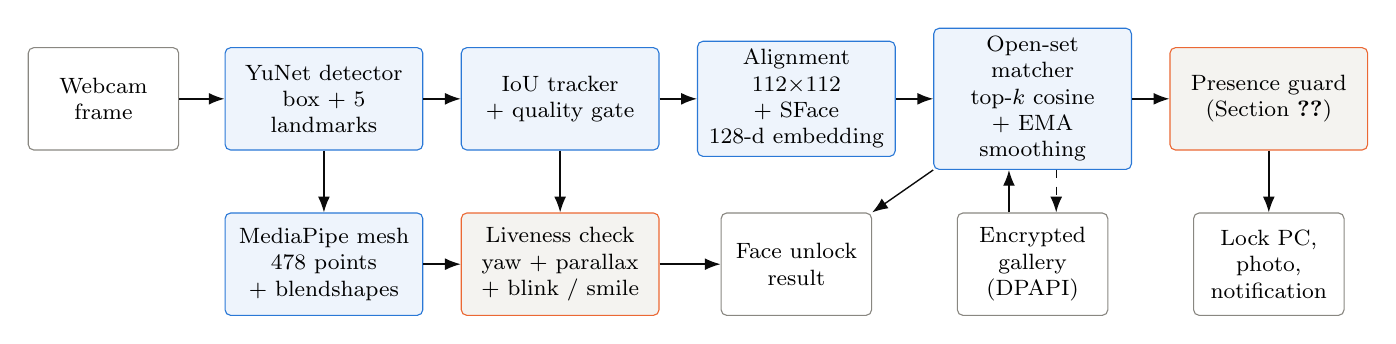
\begin{tikzpicture}[x=1mm, y=1mm,
  font=\footnotesize,
  box/.style={draw=fgblue, fill=fgfill, rounded corners=2pt, align=center, minimum height=13mm, inner sep=3pt, text width=23mm},
  sec/.style={draw=fgorange, fill=fggrey, rounded corners=2pt, align=center, minimum height=13mm, inner sep=3pt, text width=23mm},
  io/.style={draw=fgmuted, rounded corners=2pt, align=center, minimum height=13mm, inner sep=3pt, text width=17mm},
  arr/.style={-{Latex[length=2mm]}, draw=fgink, line width=0.5pt}]
\node[io]  (cam) at (0,0)   {Webcam\\ frame};
\node[box] (det) at (28,0)  {YuNet detector\\ box + 5 landmarks};
\node[box] (trk) at (58,0)  {IoU tracker\\ + quality gate};
\node[box] (emb) at (88,0)  {Alignment $112{\times}112$\\ + SFace\\ 128-d embedding};
\node[box] (mat) at (118,0) {Open-set matcher\\ top-$k$ cosine\\ + EMA smoothing};
\node[sec] (grd) at (148,0) {Presence guard\\ (Section~\ref{sec:guard})};
\node[box] (mesh) at (28,-21)   {MediaPipe mesh\\ 478 points\\ + blendshapes};
\node[sec] (live) at (58,-21)   {Liveness check\\ yaw + parallax\\ + blink / smile};
\node[io]  (unlock) at (88,-21) {Face unlock\\ result};
\node[io]  (db) at (118,-21)    {Encrypted\\ gallery (DPAPI)};
\node[io]  (os) at (148,-21)    {Lock PC, photo,\\ notification};
\draw[arr] (cam) -- (det);
\draw[arr] (det) -- (trk);
\draw[arr] (trk) -- (emb);
\draw[arr] (emb) -- (mat);
\draw[arr] (mat) -- (grd);
\draw[arr] (grd) -- (os);
\draw[arr] (det) -- (mesh);
\draw[arr] (mesh) -- (live);
\draw[arr] (trk) -- (live);
\draw[arr] (live) -- (unlock);
\draw[arr] (mat.south west) -- (unlock.north east);
\draw[arr] ([xshift=-3mm]db.north) -- ([xshift=-3mm]mat.south);
\draw[arr, dashed] ([xshift=3mm]mat.south) -- ([xshift=3mm]db.north);
\end{tikzpicture}
\caption{Architecture of \sys{}. Blue: recognition pipeline; orange: security components; gray: inputs, storage and outputs. Detection, tracking, embedding and matching run on every frame; the dense mesh is evaluated only during a liveness check or when its overlay is shown. IoU: intersection over union; EMA: exponential moving average; DPAPI: Windows Data Protection API. The dashed arrow is the bounded template update (Section~\ref{sec:adaptive}).}
\label{fig:arch}
\end{figure*}

\emph{Threat model.} We protect the unlocked OS session and, secondarily, the stored face templates against four adversaries: (A1) someone who sits down at an unattended, unlocked PC; (A2) someone at the locked PC, for instance guessing the PIN; (A3) a presentation attacker who wants face unlock to accept the owner, using a flat or bent print, a replayed recording of a genuine session, or a ``universal'' recording in which the owner performs every action; and (A4) an onlooker behind the working owner. 3-D masks, injection of synthetic video into the camera driver and malware running with the user's rights are out of scope; such malware could disable any user-level program anyway. Because \sys{} never unlocks the OS, fooling its face matcher can at worst prevent a lock or open a user-level application. Table~S1 compares the resulting functions with an idle timeout and IR-based Windows Hello sign-in.

\subsection{Recognition Pipeline}
\emph{Detection and alignment.} Each frame is scaled to a width of at most 640 pixels for YuNet (model \texttt{face\_detection\_yunet\_2023mar}), which returns a box, a confidence and five points $\mathbf{p}_1,\dots,\mathbf{p}_5$: the right and left eye centers, the nose tip, and the right and left mouth corners, as seen from the subject. The face is warped to a $112\times112$ crop by the similarity transform $(s,\mathbf{R},\mathbf{t})$ that minimizes $\sum_i \lVert s\mathbf{R}\mathbf{p}_i+\mathbf{t}-\mathbf{q}_i\rVert^2$ for canonical positions $\mathbf{q}_i$.

\emph{Embedding.} The SFace network $\mathcal{F}$ (model \texttt{face\_recognition\_sface\_2021dec}, 38.7~MB) maps the crop $\mathbf{x}$ to $\mathcal{F}(\mathbf{x})\in\mathbb{R}^{128}$. With the normalization $\nu(\mathbf{v})=\mathbf{v}/\lVert\mathbf{v}\rVert$ and $\mathrm{flip}(\cdot)$ the horizontal mirror image, enrollment and verification use flip test-time augmentation (TTA),
\begin{equation}
\mathbf{e}(\mathbf{x}) = \nu\bigl(\nu(\mathcal{F}(\mathbf{x}))+\nu(\mathcal{F}(\mathrm{flip}(\mathbf{x})))\bigr),
\end{equation}
and faces are compared by their cosine similarity $s=\mathbf{e}_a^\top\mathbf{e}_b$. Live tracking skips the mirror image to save time.

\emph{Open-set matching.} A person $p$ is enrolled with unit-norm samples $\{\mathbf{g}_{p,j}\}$, typically 22 images taken in five guided head poses. A query $\mathbf{q}$ receives the mean of its $k=3$ highest similarities to that person,
\begin{equation}
S_p(\mathbf{q})=\frac{1}{k}\sum_{j\in\mathcal{T}_k(p)}\mathbf{q}^\top\mathbf{g}_{p,j},
\end{equation}
where $\mathcal{T}_k(p)$ indexes these samples. Averaging the closest samples favors enrollment images whose pose resembles the query and is less noisy than a single nearest neighbor. The scores of a tracked face are smoothed by an exponential moving average, $\tilde{S}_p(t)=\alpha S_p(t)+(1-\alpha)\tilde{S}_p(t-1)$ with $\alpha=0.5$, and with $p^\star=\arg\max_p\tilde{S}_p$ the face is labeled
\begin{equation}
\text{label}=\begin{cases}
\text{match}, & \tilde{S}_{p^\star}\ge\tau,\\
\text{unknown}, & \tilde{S}_{p^\star}<\tau_u,\\
\text{uncertain}, & \text{otherwise,}
\end{cases}
\end{equation}
where $\tau_u=0.30$ and $\tau$ equals 0.38, 0.45 or 0.52 for the relaxed, balanced (default) and strict security levels. Alarms can be raised only by \emph{unknown} faces and unlocking needs a \emph{match}, while ambiguous frames fall in the \emph{uncertain} band.

\emph{Tracking and quality gate.} Detections are linked to tracks by intersection over union (IoU $\ge0.25$), with a fallback on center distance and size that handles fast motion at low frame rates, and each track is re-embedded every 0.35~s (0.2~s in the background). A rule-based quality gate on face size, sharpness, exposure, detector score and pose does not stop a face from being tracked and matched; it decides which faces may be enrolled, may update a template and may trigger an intruder lock. Its limits, listed in Section~S1, are deliberately conservative relative to the degradation results of Section~\ref{sec:robust}.

\subsection{Head-Pose Estimation and Roll Leakage}\label{sec:yaw}
Let $\mathbf{u}$ be the unit vector pointing from the right to the left eye, $d=\lVert\mathbf{p}_2-\mathbf{p}_1\rVert$ the distance between the eyes and $\mathbf{m}=(\mathbf{p}_1+\mathbf{p}_2)/2$ their midpoint. The estimator measures the roll $\phi=\operatorname{atan2}(u_y,u_x)$, rotates the nose offset back with the 2-D rotation matrix $\mathbf{R}_{-\phi}$, $\mathbf{n}'=\mathbf{R}_{-\phi}(\mathbf{p}_3-\mathbf{m})$, and converts it into a yaw ratio and angle
\begin{equation}
\gamma = n'_x/d,\qquad \hat{\theta}=\arctan(\gamma/K),
\end{equation}
where $K=\parKratio$ is fitted on a calibration set of real 3-D faces (Section~\ref{sec:pose}). On \poseN{} LFW photographs, $\hat\theta$ agrees with the 3-D head pose of the MediaPipe face mesh~\cite{kartynnik2019facemesh} with a Pearson correlation of \poseR{} and a mean absolute difference of \poseMae$^\circ$; the analogous pitch estimate correlates only at \posePitchR{} and is used only to guide enrollment.

Turning a flat photograph by $\beta$ about a vertical axis does more than compress it horizontally. A pinhole camera with focal length $f$ at distance $D$ images the card point $(x,y)$ at $(f x\cos\beta,\, f y)/(D+x\sin\beta)$, which enlarges the nearer side and slants the eye line by an angle $\phi_\beta\neq0$. Undoing this slant also rotates the nose offset, whose vertical part $h$ is much larger than its horizontal part, and moves roughly $h\sin\phi_\beta$ into $n'_x$. As Fig.~\ref{fig:parallax}(a) shows, the average apparent yaw of a tilted print stays small, but individual faces reach \parFlatRatioMax$^\circ$ of apparent yaw change, enough to pass a head-turn prompt.

\begin{figure*}[!t]
\centering
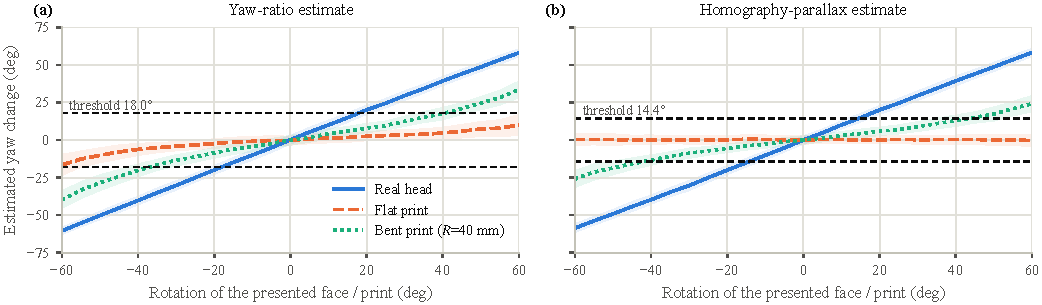
\includegraphics[width=0.9\textwidth]{figures/fig_parallax.pdf}
\caption{Estimated yaw change against the rotation of a real head, a flat print and a print bent into a cylinder of radius 40~mm, rendered from \parFacesEval{} held-out 3-D face meshes through a webcam model with 1-pixel landmark noise (mean $\pm$ s.d.; Section~\ref{sec:pose}). (a) The yaw ratio also responds to tilted prints because of roll leakage. (b) The mean homography parallax of the flat print stays near zero for every angle.}
\label{fig:parallax}
\end{figure*}

\subsection{Homography-Parallax Cue}\label{sec:parallax}
The eye centers and mouth corners lie close to one plane, whereas the nose tip sits on average \parNose~mm in front of the eye plane. Denote by $\mathbf{b}_i$ the landmarks recorded while the user looks straight at the camera, by $\mathbf{c}_i$ the current ones, and by $\mathbf{b}^{\mathrm{h}}_i=[\mathbf{b}_i^\top,1]^\top$ their homogeneous coordinates. The homography $\mathbf{H}$ with $\mathbf{c}_i\simeq\mathbf{H}\mathbf{b}^{\mathrm{h}}_i$ for $i\in\{1,2,4,5\}$, where $\simeq$ denotes equality up to scale, is obtained by the direct linear transform~\cite{hartley2004mvg}, and four correspondences determine it exactly. Mapping the baseline nose gives the prediction $\hat{\mathbf{c}}_3=\eta(\mathbf{H}\mathbf{b}^{\mathrm{h}}_3)$, where $\eta$ divides by the third coordinate, and we define the parallax ratio and the parallax yaw
\begin{equation}
\rho=\frac{(\mathbf{c}_3-\hat{\mathbf{c}}_3)^\top\mathbf{u}}{d},\qquad \psi=\arctan(\rho/K_p),
\end{equation}
with $K_p=\parKpar$ fitted on the calibration set.

\begin{proposition}
If the five landmarks lie on a plane, i.e.\ for any flat print or screen, and are observed without noise by a pinhole camera, then $\rho=0$ for every rigid motion of the plane.
\end{proposition}
\begin{proof}
A scene plane is mapped to the image by a homography, so the baseline and current views of the plane differ by some homography $\mathbf{H}_0$. Since four points in general position determine a homography uniquely, $\mathbf{H}=\mathbf{H}_0$. The nose lies on the same plane, hence $\mathbf{c}_3\simeq\mathbf{H}_0\mathbf{b}^{\mathrm{h}}_3$ and $\hat{\mathbf{c}}_3=\mathbf{c}_3$.
\end{proof}

When a real head turns, the protruding nose leaves its predicted position and $\psi$ follows the rotation (Fig.~\ref{fig:parallax}(b)). In practice landmark noise and lens distortion make $\rho$ small but nonzero for flat prints, which the acceptance threshold has to absorb (Section~\ref{sec:pose}), and a print bent into a cylinder is no longer planar and produces some parallax, although far less than a head. The test reuses the detector's landmarks and costs one $8\times8$ linear solve per frame.

\subsection{Challenge-Response Protocol}\label{sec:protocol}
A face-unlock session (Algorithm~\ref{alg:live}) passes through the phases \emph{align}, \emph{challenge}$_i$, \emph{recenter} and \emph{final}. While aligning, the user looks at the camera for four frames, and the session stores the baseline yaw $\hat\theta_0$, the baseline blink and smile scores $b_0$ and $s_0$, the baseline landmarks $\mathbf{b}_i$ and a reference embedding. It then asks for $n=3$ actions drawn without replacement from $\{$turn left, turn right, blink, smile$\}$, so every sequence contains at least one turn and one expression; without a face mesh only turns are requested, never the same one twice in a row. A turn is accepted after two consecutive frames with $\pm(\hat\theta-\hat\theta_0)\ge\tau_\theta$ and $\pm\psi\ge0.8\,\tau_\theta$, where $\tau_\theta=18^\circ$. Using the blendshape scores of the face mesh, a blink must lift the blink score above $\max(0.30,b_0+0.20)$ and let it fall below $\max(0.20,b_0+0.10)$ again, and a smile must hold the smile score above $\max(0.5,s_0+0.3)$ for two frames; the thresholds are relative to the user's baseline so that people with a high resting score are not rejected.

\begin{algorithm}[!t]
\caption{Face-unlock liveness session}\label{alg:live}
\footnotesize
\begin{algorithmic}[1]
\Require frames with landmarks, yaw $\hat\theta$, blink and smile scores, embeddings
\Ensure \textsc{pass} with an identity, or \textsc{fail} with a reason
\State record $\hat\theta_0$, $b_0$, $s_0$, $\mathbf{b}_i$ and a reference embedding over 4 frontal frames
\State draw 3 distinct actions from \{left, right, blink, smile\}; strikes $\gets 0$
\For{each action $a$}
  \State show the prompt; $t_p\gets$ now
  \Repeat
    \IfThen{2nd face, face lost $>1$~s, or identity $<0.40$ within $20^\circ$}{\Return \textsc{fail}}
    \IfThen{off-prompt action starts from neutral}{strikes $\gets$ strikes $+1$}
    \IfThen{strikes $>1$}{\Return \textsc{fail}}
    \State count $a$ only if its onset ($\kappa>0.3$) is in $[t_p{+}0.15,\,t_p{+}3.5]$~s
    \IfThen{no valid onset by $t_p{+}3.5$~s, or $a$ lasts $>7$~s}{\Return \textsc{fail}}
  \Until{$a$ is accepted}
  \State wait until the face is centered again
\EndFor
\State \Return the matcher's decision on the mean frontal embedding
\end{algorithmic}
\end{algorithm}

\emph{Order enforcement.} Performing an action that belongs to another prompt, such as turning the wrong way, turning while a blink or smile is requested, or smiling during a turn or blink prompt, earns a strike. As the reflected view may lead one to confuse left and right, the first strike is excused, but the second strike ends the session. A blink does not count as a strike at all, and an additional strike is counted only after the face has returned to a neutral position.

\emph{Response timing.} Each action has to begin as a reaction to its prompt. Let the progress $\kappa(t)\in[0,1]$ be the fraction of the acceptance threshold that has been reached; for a turn it is the smaller of the yaw-ratio and parallax fractions. A movement counts only if $\kappa$ first exceeds 0.3 between $t_{\min}=0.15$~s and $t_{\max}=3.5$~s after the prompt, and the session fails if no such onset occurs by $t_{\max}$. Since reaction times to visual stimuli measured with a high-speed camera are of the order of 0.3~s~\cite{tatsuno2016reaction}, the window starts below the fastest plausible reaction and leaves ample time for slow users. A looping video, in contrast, cannot anticipate a prompt, so movements already under way when the prompt appears, or starting too late, are ignored.

\emph{Identity continuity.} Every new embedding taken within $20^\circ$ of the baseline pose must keep a cosine similarity of at least 0.40 with the reference, well below typical genuine scores but above most impostor scores (Section~\ref{sec:verif}). Embeddings of strongly turned faces legitimately differ from a frontal one, so during a turn the tracker carries the identity, and a lost track forces a new check. A session also fails after 45~s in total.

\subsection{Presence Guard}\label{sec:guard}
The guard (state diagram in Fig.~S1, pseudocode in Algorithm~S1) analyzes four frames per second in the background. A face counts as \emph{authorized} when it matches the owner or a trusted person, and as a \emph{stranger} when, after at least two embeddings, it is unknown or matches an enrolled person who is not trusted, so that a single bad frame cannot raise an alarm. With $t_a$ the last time an authorized face was seen and $I(t)$ the keyboard and mouse idle time, the guard applies the following rules:
\begin{itemize}
\item \emph{Walk-away lock} once $\min(t-t_a,\,I(t))\ge T_a$ ($T_a=30$~s by default), announced 8~s beforehand; while the user types, the PC stays unlocked even if the face is out of view.
\item \emph{Intruder}: a stranger face that passes the quality gate and is present for $T_i=2.5$~s, with no authorized face during the last 3~s, is photographed and reported, and the PC is locked.
\item \emph{Shoulder-surfer}: an authorized user together with a stranger at least 40 pixels wide for 3~s produces a notification.
\item \emph{Lock-screen watch}: for $W$ minutes after locking (30 by default), confirmed strangers are photographed; otherwise the camera is released while the PC is locked.
\item \emph{Safety valves}: for 15~s after each unlock, intruder detections only suggest re-enrollment; at most three intruder locks are issued within 10 minutes; a camera failure never locks the PC; alerts are limited to one per minute.
\end{itemize}

\subsection{Template Adaptation, Storage and Implementation}\label{sec:adaptive}
Faces change over time. \sys{} appends a live embedding to a template only when its smoothed score reaches $\tau+0.12$, the face passes the quality gate and is near-frontal, its highest similarity to the stored samples is below 0.92 so that it adds information, and no update happened during the last 10 minutes. Adaptive samples are kept in a first-in-first-out buffer of at most $\min(30,n_e)$ entries, $n_e$ being the number of enrolled samples, so they never outnumber the enrollment. Templates, names and interface thumbnails are serialized, compressed and encrypted with the Windows Data Protection API, whose user-scope key is derived from the user's logon credentials, so the file can be decrypted only by the same user on the same machine~\cite{ms2024dpapi}; video is never stored.

The software is written in Python with OpenCV, MediaPipe and PySide6 (versions in Section~S5); the MediaPipe Face Landmarker supplies 478 points and 52 blendshape scores. Windows functions are reached through ctypes, so no administrator rights are needed, and every model is checked against a pinned SHA-256 hash. Besides the guard and face unlock, the application (Fig.~S2) offers a live view, guided enrollment and an intruder gallery, and \texttt{faceguard verify} exits with code 0 only for a live, recognized face, so it can protect user scripts. The camera is opened at $640\times480$ by default: the built-in webcam of our laptop delivered 10 frames per second at $1280\times720$ but 20 at $640\times480$, and blink detection needs the frame rate more than the resolution.

% =====================================================================================================
\section{Experimental Setup}\label{sec:setup}
\emph{Platform.} Every experiment ran on a Windows~11 laptop with an eight-core AMD Ryzen~7 7730U processor and 16~GB of memory, using the CPU only, with onnxruntime~1.30 for the baselines.

\emph{Data.} The \lfwImages{} photographs of Labeled Faces in the Wild (LFW)~\cite{huang2007lfw} show \lfwPeople{} individuals; YuNet found a face in every image, and in images with several faces the one nearest to the image center was used. For the geometry and liveness experiments we kept the first \parFaces{} of 1,500 sampled LFW images for which the MediaPipe mesh reported $|\text{yaw}|\le10^\circ$ and $|\text{pitch}|\le15^\circ$, and split their meshes at random into a calibration set of \parFacesCal{} faces, used only to fit $K$ and $K_p$, and a disjoint evaluation set of \parFacesEval{} faces, used for every geometry and liveness result. To evaluate recognition under the target condition, we use MPIIFaceGaze~\cite{zhang2017mpiifacegaze}, which contains frames recorded by the built-in webcams of \mpPeople{} participants' own laptops during everyday use over \mpDaysMin--\mpDaysMax{} days; we sampled \mpPer{} frames per participant evenly over their recording days (\mpImages{} frames, median face width \mpFacePx{} pixels).

\emph{Protocols.} Verification uses the ten View-2 splits of LFW, each holding 300 same-person and 300 different-person pairs; the threshold is fitted on nine splits and tested on the tenth. The ArcFace baselines (InsightFace models \texttt{w600k\_mbf} and \texttt{w600k\_r50}, trained on a WebFace-derived set~\cite{zhu2021webface260m}) receive the same detections and landmarks as SFace, aligned to their own canonical template, and the same flip TTA. Operating points are measured on all \opGenuine{} same-person pairs (at most 50 images per person) and on \opImpostor{} randomly drawn different-person pairs; the identification and robustness protocols are given in Section~S2. On MPIIFaceGaze, verification uses all same-person pairs recorded on different days and all different-person pairs, and the enrollment protocol of \sys{} enrolls each participant with 22 frames from their first recording days, probes with frames from the second half of their days and measures false accepts against the galleries of the other 14 participants. Every randomized step uses a fixed seed (Section~S5).

\emph{Real-world pilot.} The production code was also run on the laptop's built-in webcam ($640\times480$, about \rwFps{} frames per second) by a guided test program that stores decisions, scores, timings and, for the owner, the five landmark positions, but no images. The owner (one of the authors, enrolled with 22 images) performed face-unlock sessions with the full and the turn-only protocol and presented their own frontal photograph on a phone screen, tilting and turning it as requested, against the full protocol and against the turn-only protocol with and without the parallax gate; after every attack the owner confirmed that only the phone had been visible. A volunteer who was not enrolled attempted face unlock and took part in the guard scenarios, in which the guard used the production thresholds but only logged its decisions.

\emph{Metrics.} Verification is summarized by accuracy, the area under the receiver operating characteristic (ROC) curve (AUC), the equal error rate (EER) and the true-accept rate (TAR) at a fixed false-accept rate (FAR); the false-reject rate (FRR) is $1-\text{TAR}$. For liveness we use the terms of ISO/IEC 30107-3: APCER is the fraction of attacks accepted and BPCER the fraction of live users rejected. We report 95\% Wilson intervals, two-sided Fisher exact tests for differences between proportions, paired $t$-tests over the ten LFW folds for accuracy differences and, when no event occurs in $n$ trials, the 95\% upper bound $3/n$.

\emph{Ethics.} Apart from the public LFW and MPIIFaceGaze images and a public-domain portrait, the only human data are those of the real-world pilot, a minimal-risk feasibility test with two adult participants, one of them an author. Both gave informed consent to take part and to the publication of the anonymous results; no image or video was stored, only decisions, similarity scores, timings and, for the author, the positions of five facial landmarks. Because of its minimal risk, the pilot was not submitted to an institutional ethics committee. In deployment, photographs of strangers stay on the user's computer with a retention limit, and users should inform people who share their workspace.

% =====================================================================================================
\section{Results and Discussion}\label{sec:results}

\subsection{Verification, Baselines and Operating Points}\label{sec:verif}
Table~\ref{tab:lfw} compares SFace with two ArcFace models run through exactly the same pipeline (ROC curves in Fig.~S3). SFace reaches \lfwAccFull\% accuracy, an EER of \lfwEerFull\% and \lfwTarThreeFull\% TAR at $10^{-3}$ FAR. Both baselines perform better: the ArcFace ResNet-50 (\baseRfiftyMb~MB) reaches \baseRfiftyAcc\% (paired $t$-test against SFace: $p\pSfaceRfifty$), and the smaller ArcFace MobileFaceNet (\baseMbfMb~MB) reaches \baseMbfAcc\%, a difference that is not significant over the ten folds ($p=\pSfaceMbf$) although its EER (\baseMbfEer\%) and its TAR at $10^{-3}$ FAR (\baseMbfTarThree\%) are also better. \sys{} nevertheless uses SFace because it is distributed under the Apache~2.0 license and runs in OpenCV without further dependencies, whereas the InsightFace models are released for non-commercial research only\footnote{License terms as stated at \url{https://github.com/opencv/opencv_zoo} (SFace, Apache~2.0) and \url{https://github.com/deepinsight/insightface} (model zoo, non-commercial research purposes only), accessed Oct.~1, 2026.}; a deployment that may use them would gain accuracy after recalibrating the thresholds. Mirroring at test time lowers the EER of SFace from \lfwEerNoTTA\% to \lfwEerFull\% (accuracy gain not significant, $p=\pTta$), whereas a plain resize of the detector box instead of landmark alignment cuts the accuracy to \lfwAccNoAlign\%. Because LFW is nearly saturated and its public figures may appear in the training data of these networks, the results are best read as an upper bound.

\begin{table*}[!t]
\centering
\caption{Verification on LFW View 2 (10-Fold) Under One Protocol: Same Detections, Landmarks and Flip TTA for Every Model}
\label{tab:lfw}
\footnotesize
\setlength{\tabcolsep}{5pt}
\begin{tabular}{@{}lccccccc@{}}
\toprule
Model & Size (MB) & Time (ms)\textsuperscript{a} & Accuracy (\%) & AUC & EER (\%) & TAR (\%) @ FAR $10^{-2}$ & TAR (\%) @ FAR $10^{-3}$ \\
\midrule
\RecogRows
\midrule
SFace without flip TTA & 38.7 & -- & \lfwAccNoTTA$\pm$\lfwStdNoTTA & \lfwAucNoTTA & \lfwEerNoTTA & \lfwTarTwoNoTTA & \lfwTarThreeNoTTA \\
SFace without alignment & 38.7 & -- & \lfwAccNoAlign$\pm$\lfwStdNoAlign & \lfwAucNoAlign & \lfwEerNoAlign & \lfwTarTwoNoAlign & \lfwTarThreeNoAlign \\
\bottomrule
\end{tabular}\\[2pt]
\raggedright\scriptsize \textsuperscript{a}Embedding of one aligned $112\times112$ face including flip TTA on the laptop CPU, mean of 200 runs with each library's default threading (SFace: OpenCV DNN; ArcFace: onnxruntime).
\end{table*}

On single LFW image pairs, the FAR/FRR of the relaxed, balanced and strict levels are \farRelaxed/\frrRelaxed\%, \farBalanced/\frrBalanced\% and \farStrict/\frrStrict\% (Table~S2; score distributions in Fig.~S4). The highest of the \opImpostor{} different-person similarities was \opImpMax, and \unkImpostor\% of them fell under $\tau_u=0.30$, compared with \unkGenuine\% of the same-person pairs. The strict level thus stays below the Windows Hello limit of 0.001\% FAR~\cite{ms2024hello}, and by the rule of thumb in the same specification $10^6$ comparisons support a FAR of $10^{-5}$ at 90\% confidence. These are pairwise LFW rates, not a certification under the Windows Hello protocol, and the strict single-pair FRR exceeds the 5\% requirement, although comparing each frame with about 22 enrolled samples and smoothing over time lowers false rejections in operation. No impostor pair reached the adaptive-update gate of 0.57, which bounds the probability that an impostor frame updates a template by $3\times10^{-6}$.

\subsection{Identification and Robustness}\label{sec:robust}
Closed-set identification is \idOneNn\% correct with a single enrollment image, and trained classifiers bring no meaningful gain (Section~S2). In the open-set test (Fig.~S5, Table~S3), the top-3 rule falsely accepts \osTopthreeFarBalanced\% of unseen people at the balanced threshold, about half the rate of the nearest-neighbor rule (\osNnFarBalanced\%), while identifying \osTopthreeDirBalanced\% of enrolled probes. Under degraded probes (Fig.~S6), where clean probes give \robClean\% TAR at the balanced threshold, darkness hardly matters (\robGainLow\% TAR at 15\% brightness), whereas over-exposure does (\robGainThree\% at three times the brightness); recognition holds for faces down to about \robScaleQuarterPx{} pixels in width (\robScaleQuarter\% TAR), while detection breaks down below roughly \robScaleSmallPx{} pixels. A mask-like occluder keeps \robMask\% TAR and sunglasses \robSunglasses\%. On \robImpN{} impostor comparisons per condition, severe degradations lowered the FAR and the highest value, \robFarLargeMax\% for down-scaling by a factor of \robFarWorstLevel, remained below the pairwise FAR of the balanced level, so degraded probes are mostly rejected rather than confused with other people.

\subsection{Laptop-Webcam Images}\label{sec:webcam}
Table~\ref{tab:mpii} reports recognition on the MPIIFaceGaze frames, which resemble the use of \sys{} far more closely than LFW does: one person at a desk, a fixed built-in camera and lighting that changes over days and weeks. Across \mpGen{} same-person pairs from different days and \mpImp{} different-person pairs, SFace reaches an AUC of \mpAuc{} and an EER of \mpEer\%. At the balanced threshold \mpFarBal\% of impostor pairs were accepted and \mpFrrBal\% of genuine pairs rejected, and at the strict threshold none was accepted. Under the enrollment protocol of \sys{}, all \mpProbes{} probes from the later recording days were accepted at the balanced level and no impostor probe was (highest impostor score \mpEnrollImpMax), but at the relaxed level \mpEnrollFarRelaxed\% of impostor probes exceeded the threshold, which argues against that level when several people are enrolled. With only \mpPeople{} identities these false-accept estimates are less general than the LFW ones, but the pipeline evidently transfers to everyday laptop-webcam images and to appearance changes over weeks.

\begin{table*}[!t]
\centering
\caption{Recognition on Laptop-Webcam Images (MPIIFaceGaze, \mpPeople{} Participants, Pairs From Different Days)}
\label{tab:mpii}
\footnotesize
\setlength{\tabcolsep}{5pt}
\begin{tabular}{@{}lccccccc@{}}
\toprule
 & \multicolumn{5}{c}{Pairwise verification (cross-day)} & \multicolumn{2}{c}{Enrollment protocol, $\tau=0.45$} \\
\cmidrule(lr){2-6}\cmidrule(l){7-8}
 & & EER & TAR @ FAR & FAR @ & FRR @ & Probes & Impostors \\
Model & AUC & (\%) & $10^{-3}$ (\%) & $\tau{=}0.45$ (\%) & $\tau{=}0.45$ (\%) & accepted (\%) & accepted (\%) \\
\midrule
\MpiiRows
\bottomrule
\end{tabular}\\[2pt]
\raggedright\scriptsize -- : not applicable, because the security thresholds of \sys{} are calibrated for SFace.
\end{table*}

\subsection{Demographic Differentials}\label{sec:demo}
Table~\ref{tab:demo} reports error rates per demographic group at the balanced threshold. The groups come from the automatic attribute classifiers of Kumar \emph{et al.}~\cite{kumar2011attributes}, averaged over each person's images (\dmLabeled{} people labeled; people with ambiguous scores are left out of that attribute), and impostor pairs are drawn within each group, the harder and more relevant case~\cite{drozdowski2020bias}. The pipeline is not demographically balanced. Women have a \dmSexFmrRatio{} times higher false-match rate (FMR) and a \dmSexFnmrRatio{} times higher false-non-match rate (FNMR) than men, and the FMR among people labeled Black is about \dmEthFmrRatio{} times that among people labeled White, with people labeled Asian in between. The confidence intervals exclude chance as an explanation; only the group labeled Indian is too small to judge. Such differentials, widely reported for face recognition trained on web data~\cite{drozdowski2020bias}, are inherited here from the pretrained network and matter mainly for the guard, because a higher FMR within a group makes it more likely that a stranger is taken for an enrolled person of the same group. A balanced benchmark is needed to confirm the magnitudes, since LFW is dominated by White men and the labels are estimates.

\begin{table*}[!t]
\centering
\caption{Error Rates per Demographic Group on LFW at $\tau=0.45$ (\%; 95\% Wilson Intervals in Brackets)}
\label{tab:demo}
\footnotesize
\setlength{\tabcolsep}{6pt}
\begin{tabular}{@{}lrrcrc@{}}
\toprule
Group & People & Genuine pairs & FNMR (\%) & Impostor pairs (within group) & FMR (\%) \\
\midrule
\DemoRows
\bottomrule
\end{tabular}\\[2pt]
\scriptsize Groups from automatic attribute estimates~\cite{kumar2011attributes}.
\end{table*}

\subsection{Pose and Parallax Geometry}\label{sec:pose}
To examine both cues with known ground-truth rotation, we reconstructed the 478-point meshes described in Section~\ref{sec:setup}, removed the head pose of each photograph by rotation-only Procrustes alignment to the mean shape, scaled each mesh to an eye distance of 63~mm and rendered it with a pinhole camera ($f=457$~pixels, i.e.\ a 640-pixel image with a $70^\circ$ field of view) at 50~cm, adding 1-pixel noise to the five landmarks. Every face was rendered as a real head turned by $\beta$, as a flat print and as prints bent into cylinders of radius 60, 40 and 30~mm, all rotated by the same $\beta\in[-60^\circ,60^\circ]$. Fitting the head rotations within $\pm30^\circ$ of the \parFacesCal{} calibration faces gave $K=\parKratio$ and $K_p=\parKpar$; the same fit on the \parFacesEval{} evaluation faces gives \parKratioEval{} and \parKparEval{}, so the constants do not depend on the faces they were fitted on. On the evaluation faces, a $25^\circ$ head turn reads $\parHeadRatioTwentyFive^\circ$ from the yaw ratio and $\parHeadParTwentyFive^\circ$ from the parallax (Fig.~\ref{fig:parallax}).

For flat prints the yaw ratio reached \parFlatRatioMax$^\circ$ of apparent yaw change, whereas the parallax never exceeded \parFlatParMax$^\circ$ (99th percentile \parFlatParQ$^\circ$), which is landmark noise below the $14.4^\circ$ parallax threshold. Bent prints produce some parallax, but far less than heads: at $25^\circ$ they read \parBentSixtyParTwentyFive$^\circ$, \parBentFortyParTwentyFive$^\circ$ and \parBentThirtyParTwentyFive$^\circ$ for radii of 60, 40 and 30~mm, compared with \parHeadParTwentyFive$^\circ$ for a head, and they cross the threshold only at extreme angles that also foreshorten the face.

\subsection{Liveness Evaluation}\label{sec:liveres}
Public attack datasets do not contain free head motion in response to prompts, so we tested the protocol by Monte-Carlo simulation of the production code. Landmarks were rendered at 20 frames per second from the evaluation meshes, with subjects 40--70~cm from the camera and a lateral offset of up to 4~cm, and blink and smile scores were simulated. Simulated users reacted after log-normal delays (median 0.7~s, longer than simple visual reaction times~\cite{tatsuno2016reaction} to allow for reading the prompt), turned by $30^\circ\pm8^\circ$, turned further or blinked harder when the progress bar stalled, blinked spontaneously and mixed up left and right in 5\% of turn prompts. The print attacker tilted the photograph towards the requested side up to a random limit between $40^\circ$ and $75^\circ$. The replay attacker looped a recording of the owner completing one random sequence, and the universal-replay attacker looped a recording in which the owner cycles through all four actions; ablations used \livNAbl{} live sessions each.

\emph{Comparison with conventional protocols.} Table~\ref{tab:baselines} evaluates three conventional protocols in the same simulation: three head turns checked with the yaw ratio only, a single blink prompt in the spirit of~\cite{pan2007eyeblink}, and three random actions checked with the yaw ratio but without order enforcement or timing. The head-turn protocol accepts every live user but also \lbYawFlat\% of tilted flat prints and \lbYawBent\% of bent prints. Expression prompts stop prints, but all three conventional protocols are vulnerable to replay: a universal recording passes \lbUniMin\%--\lbUniMax\% of their sessions and a recording of one genuine session \lbRepMin\%--\lbRepMax\%. \sys{} rejects every print and lowers these rates to \lbFgUni\% (95\% interval \attUniversalFullLo--\attUniversalFullHi\%) and \lbFgReplay\% at a BPCER of \lbFgLive\%, slightly higher than that of the baselines (\lbYawLive--\lbBlinkLive\%).

\begin{table}[!t]
\centering
\caption{Liveness Protocols in One Simulation: BPCER of Live Users and APCER of Attacks (\%)}
\label{tab:baselines}
\footnotesize
\setlength{\tabcolsep}{2.4pt}
\begin{tabular}{@{}lccccc@{}}
\toprule
Protocol & BPCER & Flat & Bent & Replay & Universal \\
 & & print & $R{=}40$ & & replay \\
\midrule
\BaselineRows
\bottomrule
\end{tabular}\\[2pt]
\raggedright\scriptsize 1,000 sessions per baseline cell (\sys{}: \livN{} live, \attPrintN{} print, \attReplayN{} replay and \attUniversalN{} universal); 95\% Wilson half-widths are at most \ciHalfLive{} (BPCER), \ciHalfReplay{} (replay) and \ciHalfUniversal{} (universal) points.
\end{table}

\emph{Prints.} No print passed the full protocol (Table~\ref{tab:prints}), because a photograph cannot blink, smile or create parallax, and every sequence includes an expression. With zero successes in \attPrintN{} attempts, the APCER of each instrument is below \attPrintBound\% at 95\% confidence. The turn-only columns isolate the parallax gate: without it, tilted flat prints succeed in \attFlatTurnsOnlyNoParallax\% of sessions through roll leakage, and with it in \attFlatTurnsOnly\%. Bent prints pass turn-only sessions in \attBentRSixtyTurnsOnly\%--\attBentRThirtyTurnsOnly\% of cases because bending produces real parallax, so expression prompts remain necessary.

\begin{table}[!t]
\centering
\caption{Print Attacks: APCER (\%) Against an Adaptive Attacker Who Tilts the Print Towards the Requested Side}
\label{tab:prints}
\footnotesize
\setlength{\tabcolsep}{3pt}
\begin{tabular}{@{}lccc@{}}
\toprule
Presentation & Full & \multicolumn{2}{c}{Turn challenges only} \\
 & protocol & with parallax & without parallax \\
\midrule
\PrintRows
\bottomrule
\end{tabular}
\end{table}

\emph{Replay and ablations.} Table~\ref{tab:replay} removes one defense at a time. Against a universal replay, either defense alone is effective: the success rate falls from \attUniversalNoOrderNoTiming\% with neither to \attUniversalNoTiming\% with order enforcement only and \attUniversalNoOrderEnforcement\% with response timing only, and to \attUniversalFull\% with both (Fisher exact tests against neither, order enforcement only and timing only: $p\pUniFullNeither$, $p\pUniFullNoTiming$ and $p\pUniFullNoOrder$). Order enforcement also lowers the success of a looped genuine recording from \attReplayNoOrderEnforcement\% to \attReplayFull\% ($p=\pRepFullNoOrder$), whereas the smile rule adds little. Shortening the response window to 2.5~s reduces universal replay to \attUniversalWindowShort\% ($p\pUniShortWindow$) but rejects \livFrrWinShort\% instead of \livFrr\% of live users. No challenge-response scheme can exclude replay completely, since a recording that happens to show the requested actions at suitable times is effectively a live performance. Three distinct actions out of four give \seqDistinct{} possible sequences (min-entropy \seqMinEnt{} bits), against only \seqDistinctTurns{} in turn-only mode.

\begin{table}[!t]
\centering
\caption{Ablation of the Protocol: BPCER of Simulated Live Users and APCER of Replay Attacks (\%)}
\label{tab:replay}
\footnotesize
\setlength{\tabcolsep}{2.5pt}
\begin{tabular}{@{}lccc@{}}
\toprule
Configuration & BPCER & Replay of & Universal \\
 & (live users) & recording & replay \\
\midrule
Full protocol ($t_{\max}=3.5$~s) & \livFrr & \attReplayFull & \attUniversalFull \\
\quad without response timing & \livFrrNoTiming & \attReplayNoTiming & \attUniversalNoTiming \\
\quad without smile rule & \livFrrNoSmile & \attReplayNoSmileRule & \attUniversalNoSmileRule \\
\quad without order enforcement & \livFrrNoOrder & \attReplayNoOrderEnforcement & \attUniversalNoOrderEnforcement \\
\quad without order enf.\ and timing & n.e. & n.e. & \attUniversalNoOrderNoTiming \\
\quad without parallax gate & \livFrrNoPar & n.e. & n.e. \\
\quad response window $t_{\max}=2.5$~s & \livFrrWinShort & \attReplayWindowShort & \attUniversalWindowShort \\
\quad response window $t_{\max}=5.0$~s & \livFrrWinLong & \attReplayWindowLong & \attUniversalWindowLong \\
Turn challenges only & \livFrrTurns & \attReplayTurnsOnly & n.e. \\
\bottomrule
\end{tabular}\\[2pt]
\raggedright\scriptsize n.e.: not evaluated, because the defense does not act on that attack (parallax gate vs.\ replays of a real head) or the configuration is covered by Table~\ref{tab:baselines}. 95\% Wilson half-widths: at most \ciHalfLive{}, \ciHalfReplay{} and \ciHalfUniversal{} points for the three columns.
\end{table}

\emph{Live users.} Live users were rejected in \livFrr\% of sessions (95\% interval \livFrrLo--\livFrrHi\%), and a session lasted \livTime~s on average (95th percentile \livTimeQ~s). The parallax gate did not change the BPCER (\livFrrNoPar\% without it, $p=\pParallaxBpcer$), but response timing did: without it no live user was rejected (\livFrrNoTiming\%, $p\pTimingBpcer$), so the timing rule, which mainly targets replay, causes most of the remaining false rejections. Varying the behavioral model (Table~S4) leaves the BPCER unchanged for median reaction delays of 0.5 and 1.0~s, but it rises to \sensReactSlowest\% for very slow users (1.4~s), \sensAmpSmall\% for timid turns of $22^\circ$ and \sensConfTwenty\% when left and right are confused in 20\% of prompts; with 2-pixel landmark noise it is \livFrrNoise\% (Fig.~S7).

\subsection{Presence Guard}\label{sec:guardres}
The guard was run with the production engine and thresholds on simulated 4-frame-per-second webcam streams, made by pasting LFW photographs into $640\times480$ frames with random shifts, gain changes and sensor noise. In the \emph{owner at the desk} scenario, \gOwners{} people with at least 20 images were enrolled with 10 images each and then shown their remaining photographs for 1--6~s each, \gMinutes{} minutes per owner, a harder task than facing a webcam at a fixed desk. The owner was recognized in \gMatchFrac\% of \gFrames{} frames (Table~S5), and neither a false intruder lock nor a walk-away lock occurred in \gHours{}~h without typing, which bounds the false-lock rate by \gLockBound{} per hour. The \gShldAlerts{} shoulder-surfer alerts were traced to the \gdSecondPct\% of images in which a second, unknown person at least 40~pixels wide is visible, a common sight in news pictures; they are correct under the rule but show that it flags anyone in view.

A stranger who sat down 5~s after the owner had left was locked out within 20~s in \gIntrRate\% of \gIntrN{} trials, after a median of \gIntrMed~s (95th percentile \gIntrQ~s), i.e.\ the 2.5~s confirmation plus the first embeddings. A stranger who replaced the owner without a gap was locked out in \gReplRate\% of trials, with the 95th percentile growing to \gReplQ~s because of the 3~s rule on authorized faces, and onlookers were reported in \gShldRate\% of \gShldN{} trials after a median of \gShldMed~s. Each miss in the intruder and onlooker trials occurred because the quality gate rejected the photograph or the score fell in the uncertain band; no stranger was ever accepted as the owner. The guard thus trades a few missed strangers for the absence of false locks, the right balance for a tool that must never lock out its owner.

\subsection{Real-World Pilot}\label{sec:pilot}
A first run with the earlier protocol (\rwPilotTrials{} sessions) immediately exposed faults that the simulation had missed: only \rwPilotOwnerPass{} of the owner's \rwPilotOwner{} genuine face-unlock sessions passed. In \rwPilotDiff{} sessions the identity check rejected the owner, who had turned their head by $31^\circ$--$49^\circ$, where the embedding of a real face differs from the frontal reference; in \rwPilotBlink{} sessions natural blinks were missed because, at the 10 frames per second that the webcam delivered at $1280\times720$, a blink was sampled at peak scores of only 0.23--0.39 (the blink thresholds were then 0.45 and 0.25); and in \rwPilotNoResp{} sessions the owner did not start the requested turn within 3.5~s. We corrected the first two faults (identity check within $20^\circ$ of the baseline pose, blink thresholds 0.30 and 0.20, camera at $640\times480$), kept the response window, re-ran the liveness simulations with the corrected protocol (Section~\ref{sec:liveres}) and repeated the pilot (Table~\ref{tab:pilot}).

\begin{table}[!t]
\centering
\caption{Real-World Pilot With the Laptop Webcam (Corrected Protocol; 95\% Wilson Intervals in \%)}
\label{tab:pilot}
\footnotesize
\setlength{\tabcolsep}{2.5pt}
\begin{tabular}{@{}lcl@{}}
\toprule
Condition & Trials & Outcome \\
\midrule
\PilotRows
\bottomrule
\end{tabular}\\[2pt]
\raggedright\scriptsize Guard in log-only mode with the production thresholds. Cue: the owner leaves (walk-away, stranger, locked PC) or the volunteer steps behind the owner (shoulder-surfer).
\end{table}

The owner passed \rwOwnerPass{} of \rwOwnerN{} live sessions at about \rwFps{} frames per second with a genuine similarity of about \rwOwnerSim; the one failure was again a late response. The volunteer was never accepted as the owner (similarity \rwVolSim) but passed the liveness check in only \rwVolLive{} of \rwVolN{} sessions, failing twice by turning the wrong way, so first-time users can confuse left and right in a mirrored preview and need a clearer cue, such as an arrow. None of the \rwAttN{} phone-screen attacks was accepted (95\% upper bound \rwAttUpper\%). By tilting the phone, however, the attacker produced at most \rwAttYawMax$^\circ$ of apparent yaw change and \rwAttParMax$^\circ$ of parallax, against a median parallax of \rwOwnerParMed$^\circ$ for genuine turns; the attacks failed before the parallax gate became decisive, and the strongly tilted print of Section~\ref{sec:pose} remains to be reproduced physically. The guard locked the PC \rwWalkBeep~s after the owner walked away, alerted to the onlooker \rwShldBeep~s after the cue and photographed the volunteer at the locked PC \rwLockwBeep~s after the owner left. A stranger who sat down was locked out \rwIntrLat~s after first being detected, much later than in the simulation, because the volunteer's live scores repeatedly fell into the uncertain band between 0.30 and 0.45, which interrupts the 2.5~s confirmation of an unknown face. These few trials demonstrate feasibility and expose failure modes, but they cannot support rate estimates.

\subsection{Runtime}\label{sec:runtime}
At the default $640\times480$ resolution, detection takes \rtDet~ms and one embedding \rtEmb~ms, or \rtEmbTta~ms with mirroring (Fig.~S8). A frame of the complete pipeline costs \rtPipe~ms on average and \rtPipeMesh~ms with the face mesh. The live view ran at \rtFps{} frames per second with a total CPU load of \rtCpuLive\%, and the background guard used \rtCpuGuard\%. The ArcFace MobileFaceNet would also be the fastest embedding (Table~\ref{tab:lfw}) where its license permits.

\subsection{Discussion and Limitations}\label{sec:discussion}
\emph{Security position.} \sys{} only adds protection: a false reject locks a present owner, who then enters the PIN, and a false accept prevents a lock, leaving the OS as it would have been without \sys{}. The safety valves prevent lock-out loops, and encrypted templates without stored video limit the privacy exposure.

\emph{Liveness.} The parallax gate removes the tilted-print weakness of the yaw ratio, and order enforcement with response timing makes universal replay several times less successful than in conventional protocols. RGB-only challenge-response still cannot stop a replay that happens to match the prompts, bent prints in turn-only mode, 3-D masks or injected video, so sensitive resources should add IR or depth sensing or a passive learned detector (Section~\ref{sec:related}). Proposition~1 assumes an ideal pinhole camera; the radial distortion of wide-angle webcams adds a small parallax to flat prints, which the threshold must absorb or a calibrated undistortion step would remove.

\emph{Validity.} The rate estimates for liveness and the guard come from simulation with rendered landmarks, a behavioral model and composited photographs. The held-out calibration and the sensitivity analysis show that the conclusions do not hinge on the fitted constants or on a particular behavioral setting, and the pilot confirmed the qualitative behavior, but it also showed what simulation misses: real users turn further and react later than modeled, low frame rates blunt blinks, first-time users confuse left and right, and live impostor scores can hover in the uncertain band. With two participants and only phone-screen attacks, a study with many participants and physical print, replay and mask instruments, reporting APCER and BPCER per instrument, remains the most important next step. The webcam evaluation used only 15 identities, and the demographic analysis relies on estimated labels on an unbalanced dataset.

% =====================================================================================================
\section{Conclusion}\label{sec:conclusion}
This paper presented \sys{}, a CPU-only system that adds face recognition, liveness checks and continuous presence authentication to ordinary webcams while leaving OS sign-in untouched. Its permissively licensed SFace pipeline achieves \lfwAccFull\% accuracy on LFW, slightly below ArcFace models under the same protocol, and an EER of \mpEer\% on laptop-webcam images recorded over weeks, but its false-match rates differ substantially between demographic groups. We showed that perspective-induced roll leakage lets tilted prints pass five-landmark head-turn checks and proposed a homography-parallax cue that vanishes for planar presentations. Combined with ordered and timed challenges, it stopped every simulated print attack and reduced replay success well below that of conventional protocols, although replays of the genuine user remain a limit of RGB-only liveness. A real-world pilot rejected every phone-screen attack and revealed two faults that simulation had missed, which we corrected. Future work includes a study with many participants and physical attack instruments, a demographically balanced evaluation with mitigations such as group-aware thresholds, and passive presentation-attack models.

\section*{Acknowledgment}
We thank the pilot volunteer, the creators of LFW, MPIIFaceGaze and the LFW attribute labels, and the OpenCV Model Zoo, MediaPipe and InsightFace teams for publishing their data and models. In accordance with the IEEE policy on AI-generated content, we disclose that an AI system (Claude, Anthropic) was used to write the software and the experiment scripts, to generate the figures, and to draft the text of all sections, figure captions and tables of this manuscript. The authors reviewed and edited the text, checked the code and verified every reported result, and they take full responsibility for the content.

\bibliographystyle{IEEEtran}
\bibliography{references}

\end{document}
